\chapter{Digitalização das áreas-meio e fim do Poder Judiciário}

O Brasil pós-democrático foi implementado como uma república  federativa, em concordância com \cite{cf88}, formada pela união indissolúvel dos Estados e Municípios e do Distrito Federal, constitui-se em Estado Democrático de Direito, cujos Poderes são o Executivo, Legislativo e Judiciário.

Haja vista o foco deste trabalho é o Poder Judiciário, esse Poder é composto, segundo \cite{cf88}, no art. 92 da Constituição Federal:

\begin{itemize}
    \item Supremo Tribunal Federal.
    \item Conselho Nacional de Justiça.
    \item Superior Tribunal de Justiça.
    \item Tribunais Regionais Federais e Juízes Federais.
    \item Tribunais e Juízes do Trabalho.
    \item Tribunais e Juízes Eleitorais.
    \item Tribunais e Juízes Militares.
    \item  Tribunais e Juízes dos Estados e do Distrito Federal e Territórios.
\end{itemize}

\cite{cf88} concedeu ao Poder Judiciário autonomia administrativa e financeira. A importância da autonomia para o Poder Judiciário se confirma ao analisar as figuras seguintes relativas ao controle judicial sob o Poder Executivo,  corrupção no Poder Judiciário, Estado de Direito e a corrupção política.

A figura \ref{fig:judicial-constraints-on-the-executive-index} mostra a situação mundial do controle judicial sobre o Poder Executivo em 2024.

\begin{figure}[H]
	\centering
	\caption{Índice de controle judicial sobre o Poder Executivo}
	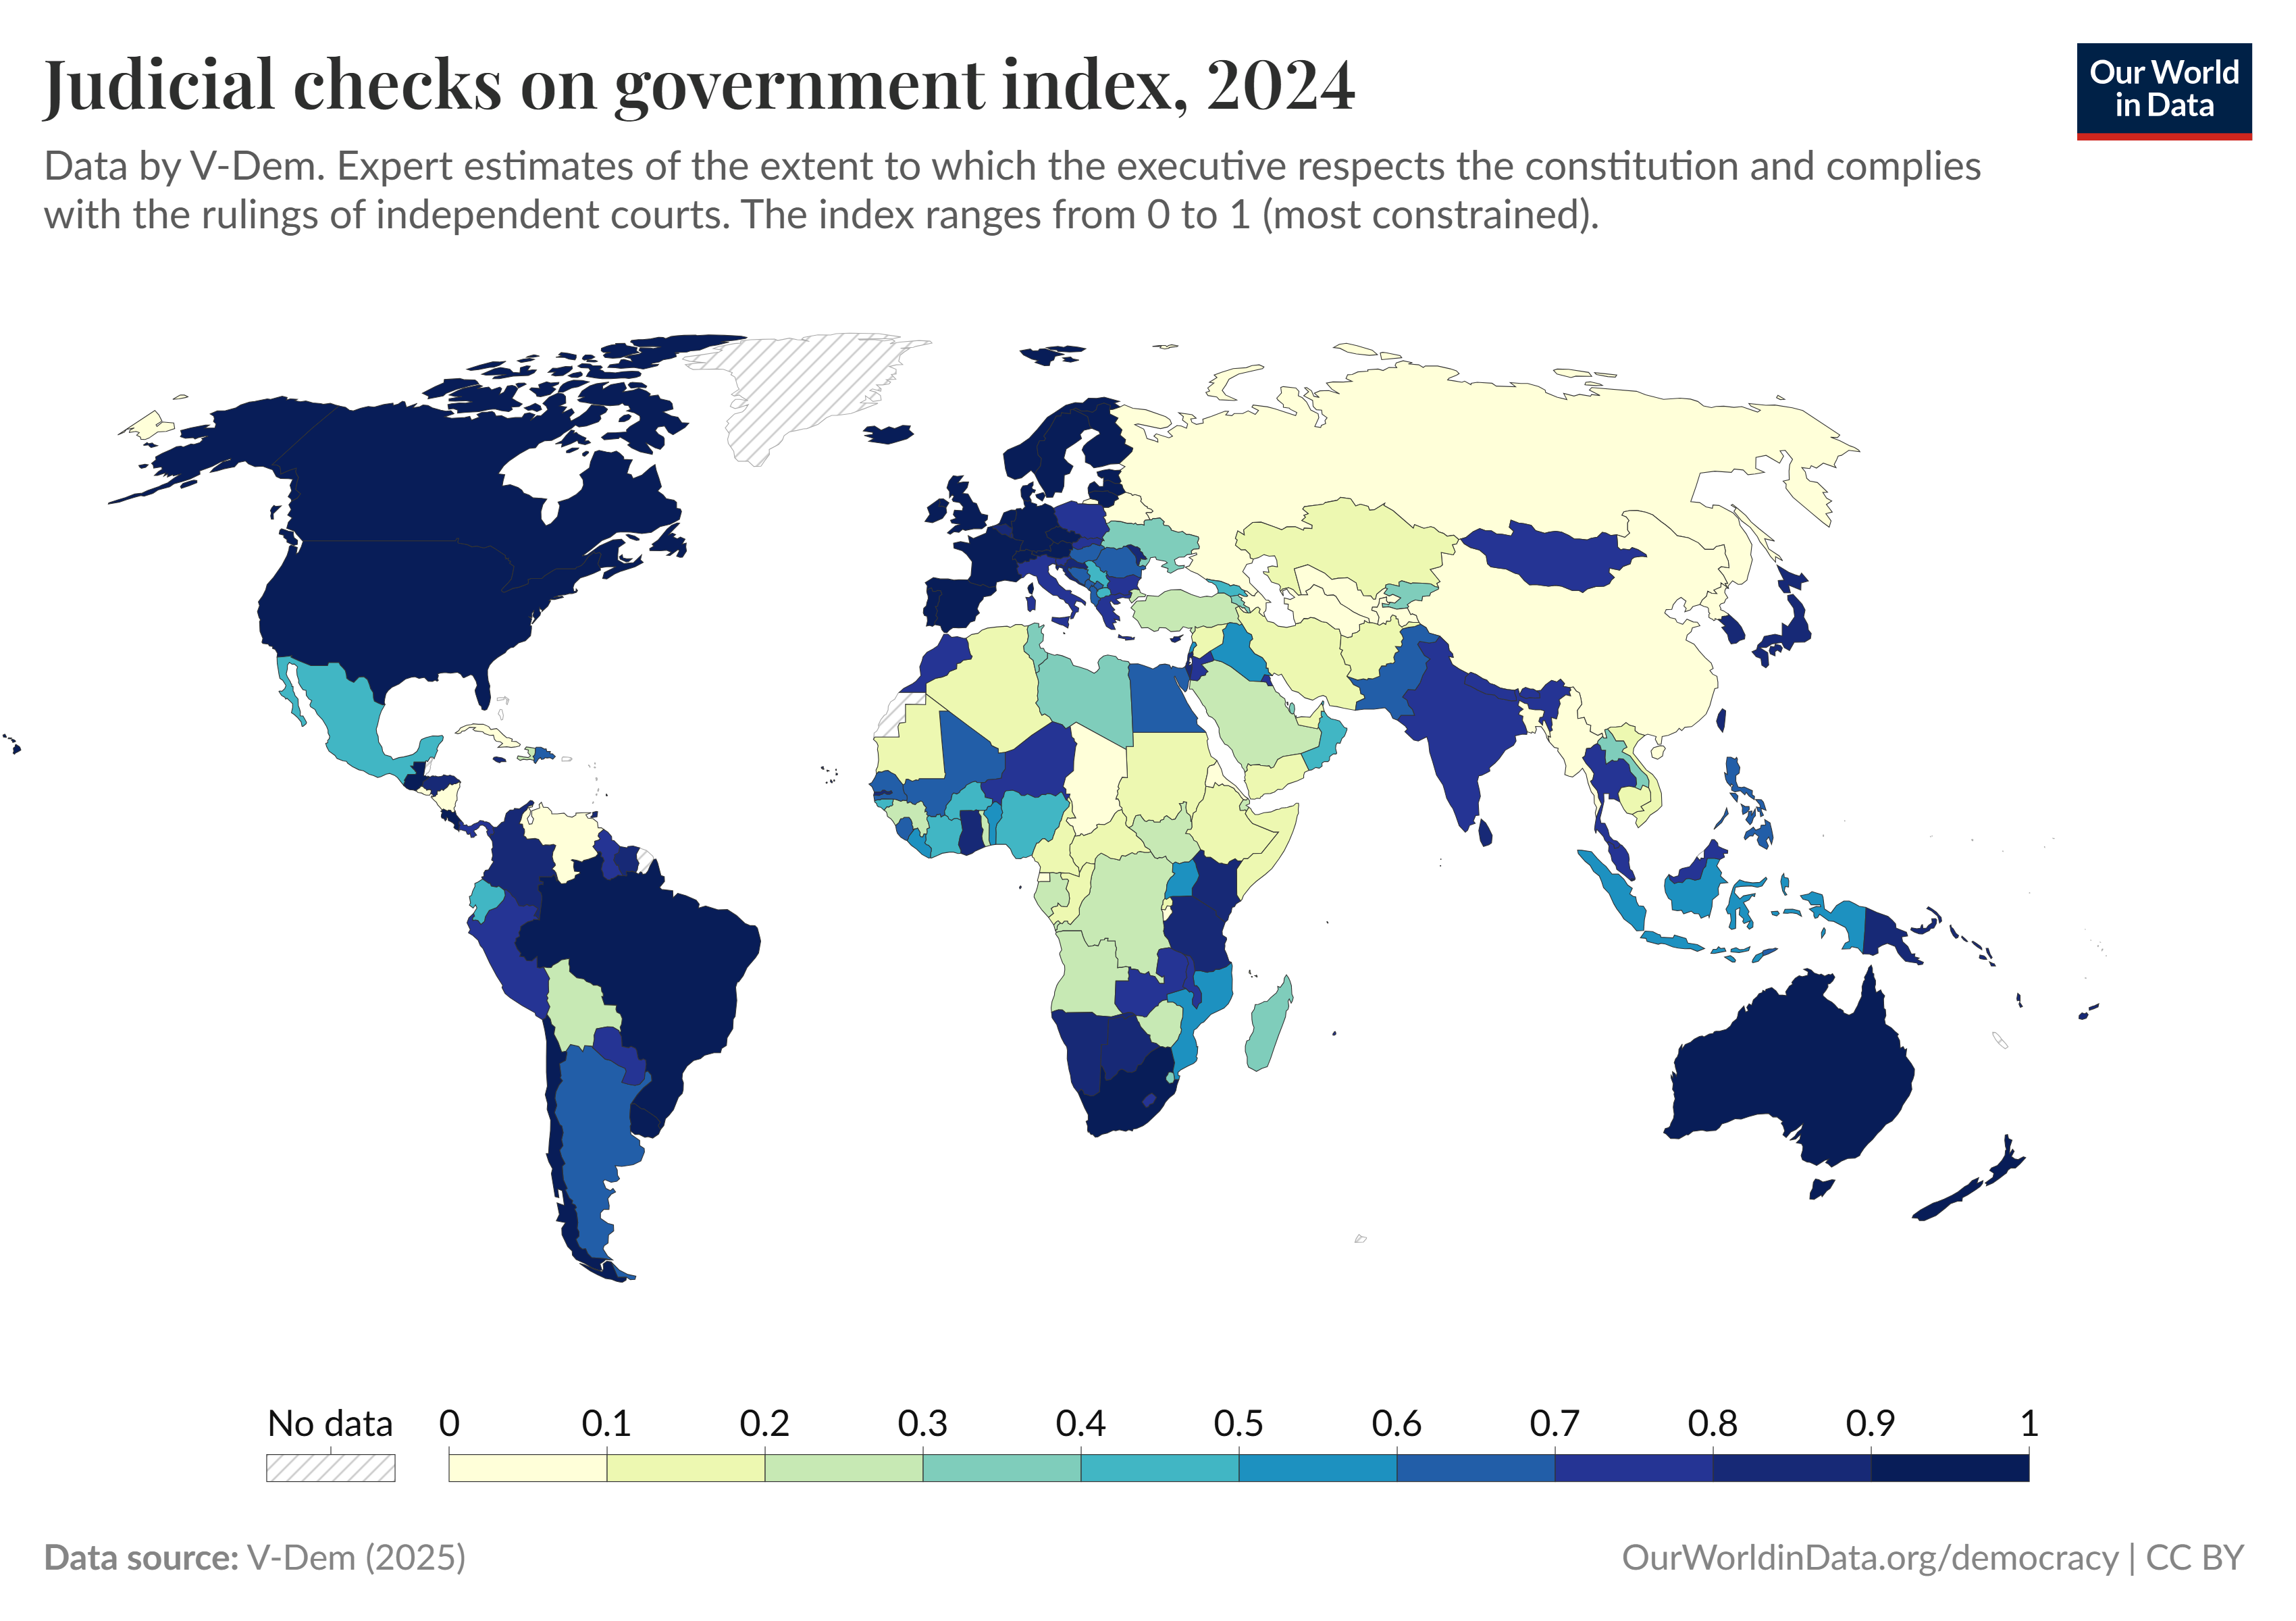
\includegraphics[width=1\linewidth]{figuras/judicial-constraints-on-the-executive-index}
	\label{fig:judicial-constraints-on-the-executive-index}
	\footnotesize{Fonte: \cite{jus_constraints_on_gov}.}
\end{figure}

Nota-se como o Poder Judiciário tem pouquíssimo controle sobre o Poder Executivo na em uma quantidade grande de países. A figura detalha o referido controle judicial no Brasil desde 1822 até 2024.

\begin{figure}[H]
    \centering
    \caption{Índice de controle judicial sobre o Poder Executivo no Brasil (1822-2024)}
    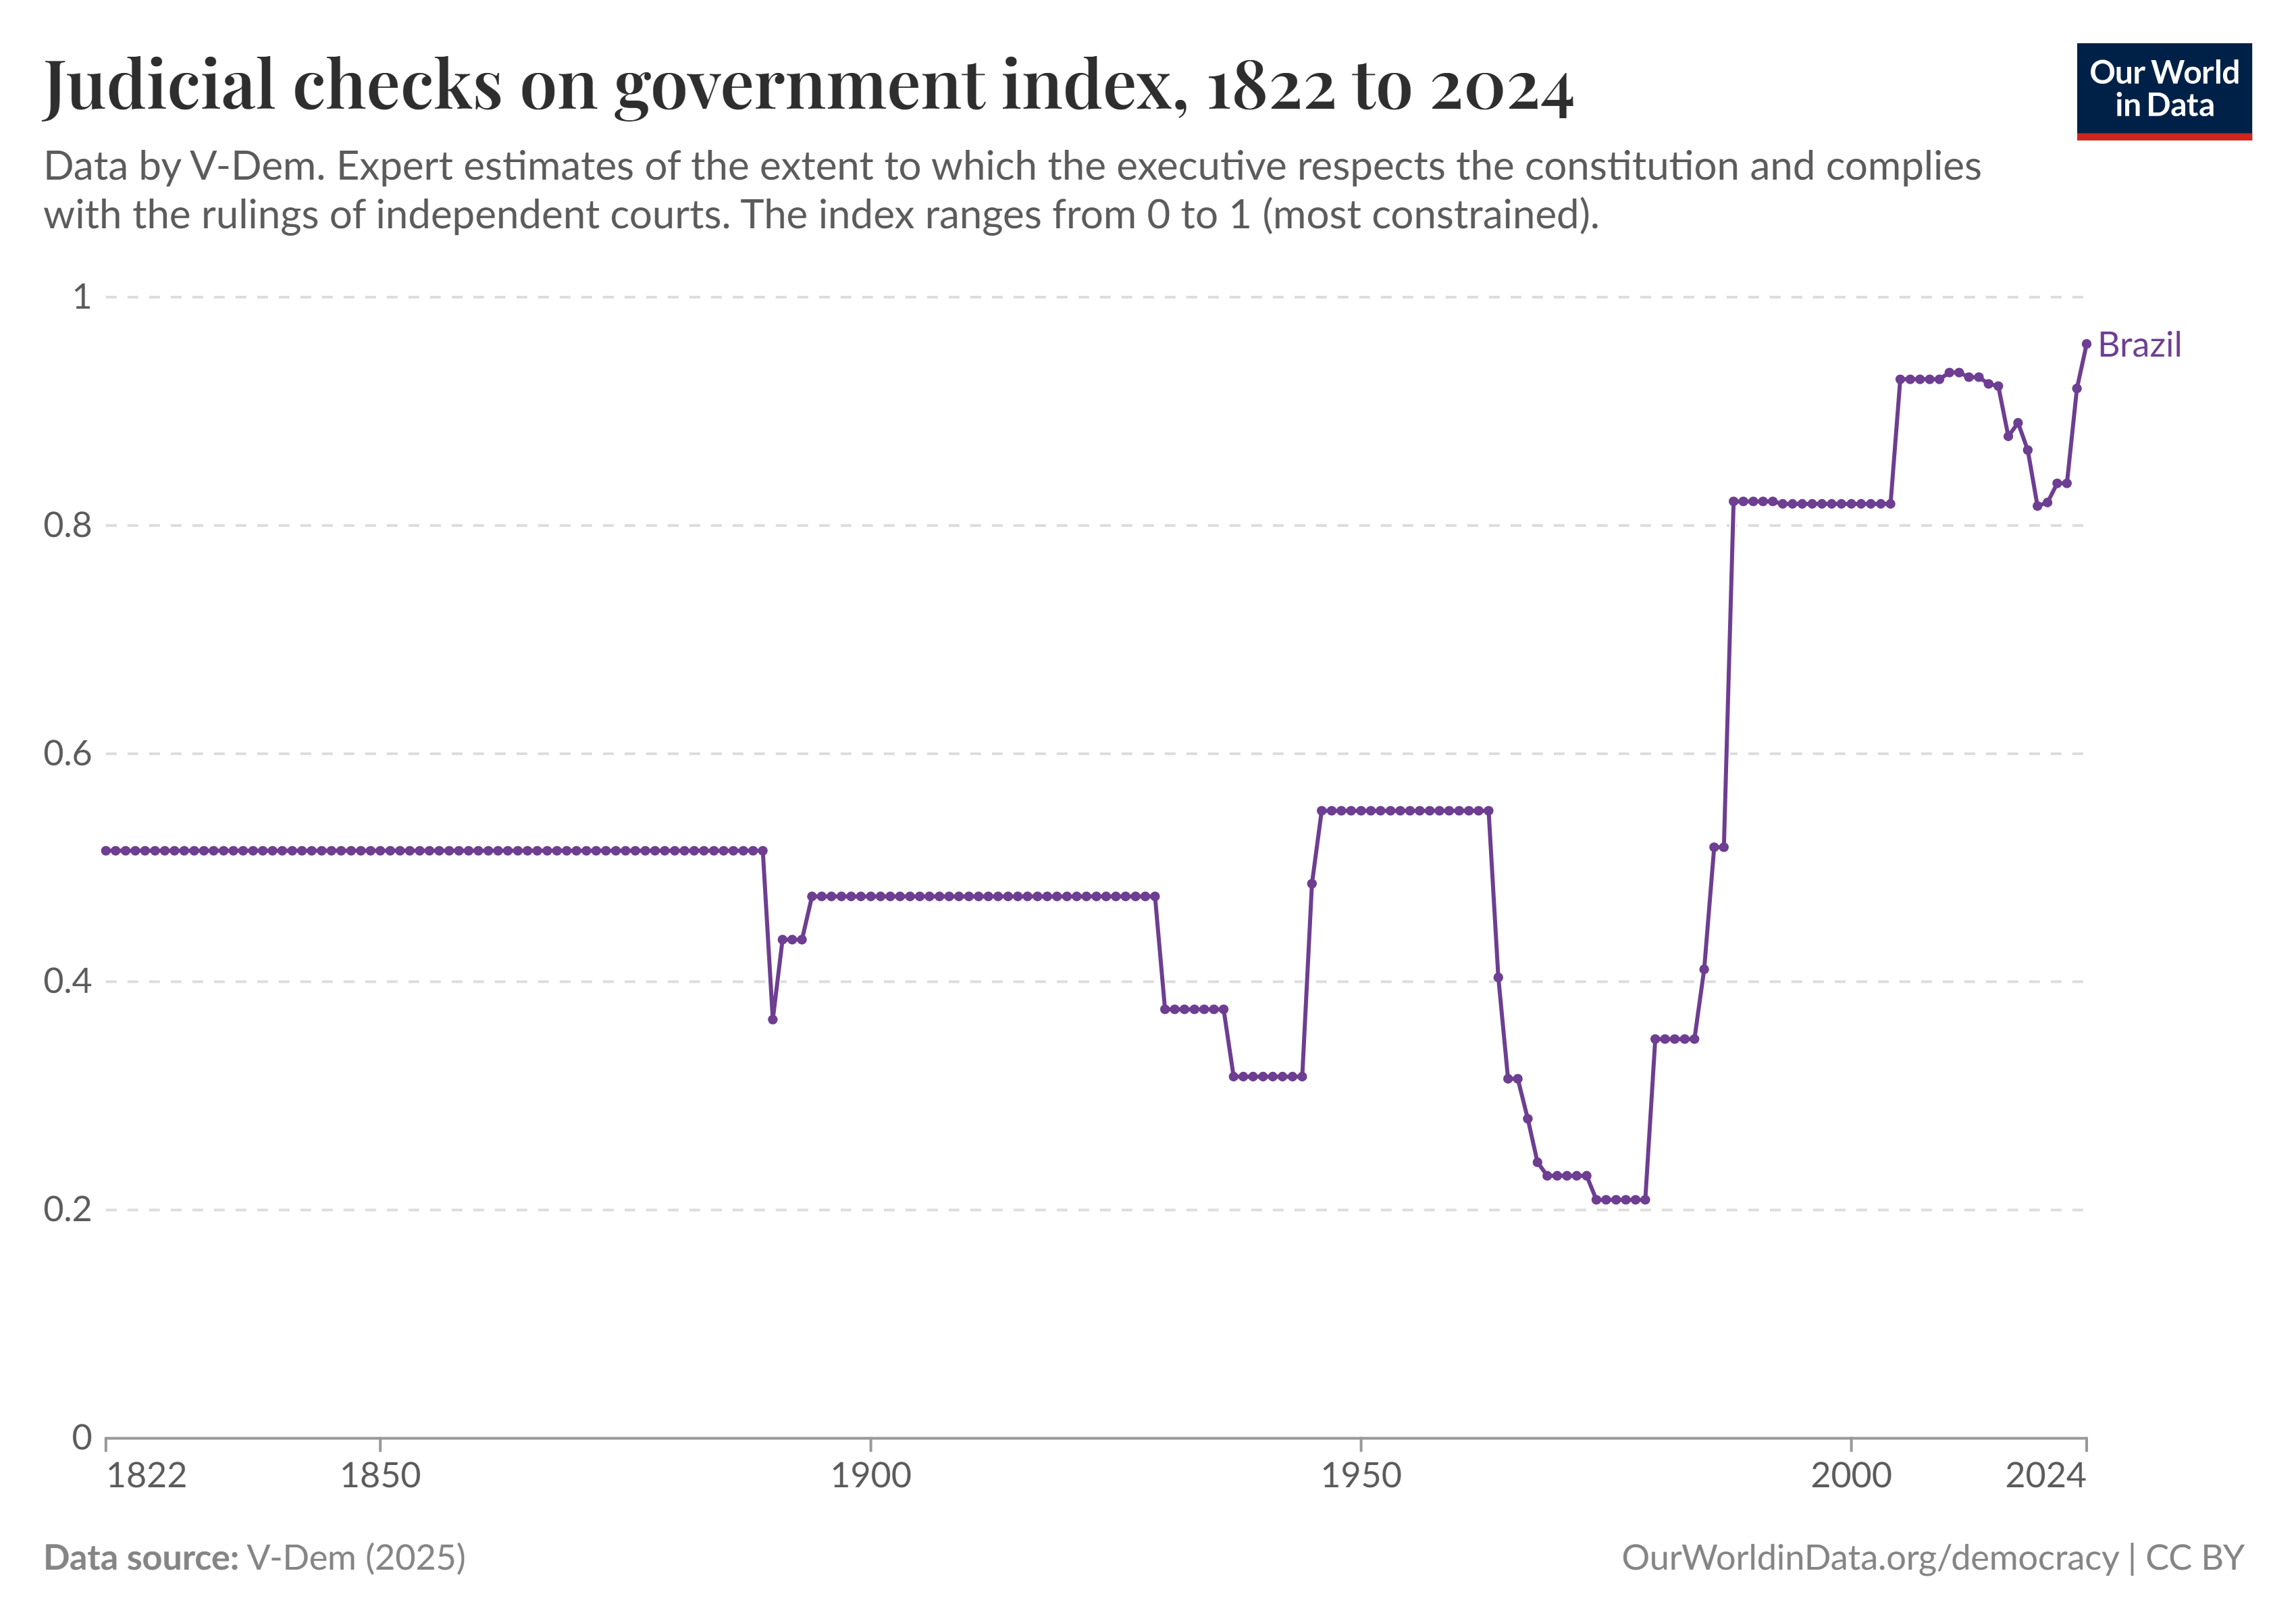
\includegraphics[width=1\linewidth]{figuras/judicial-constraints-on-the-executive-index-brazil}
    \label{fig:judicial-constraints-on-the-executive-index-brazil}
    \footnotesize{Fonte: \cite{jus_constraints_on_gov}.}
\end{figure}

No tocante a figura \ref{fig:judicial-constraints-on-the-executive-index-brazil}, nota-se como a democracia melhorou os índices do Brasil. Em 2024, o Brasil quase atingiu o valor máximo - 0,96 - enquanto a média mundial foi 0,664. Apenas 31 países de 193 - equivalente a 16\% do total - alcançaram uma pontuação de, no mínimo, 0,9 de 1,0 até o máximo.

A figura \ref{fig:quartis_controle_jus_sobre_gov} contém o Índice de controle judicial sobre o Poder Executivo.

\begin{figure}[H]
    \centering
    \caption{Índice de controle judicial sobre o Poder Executivo}
    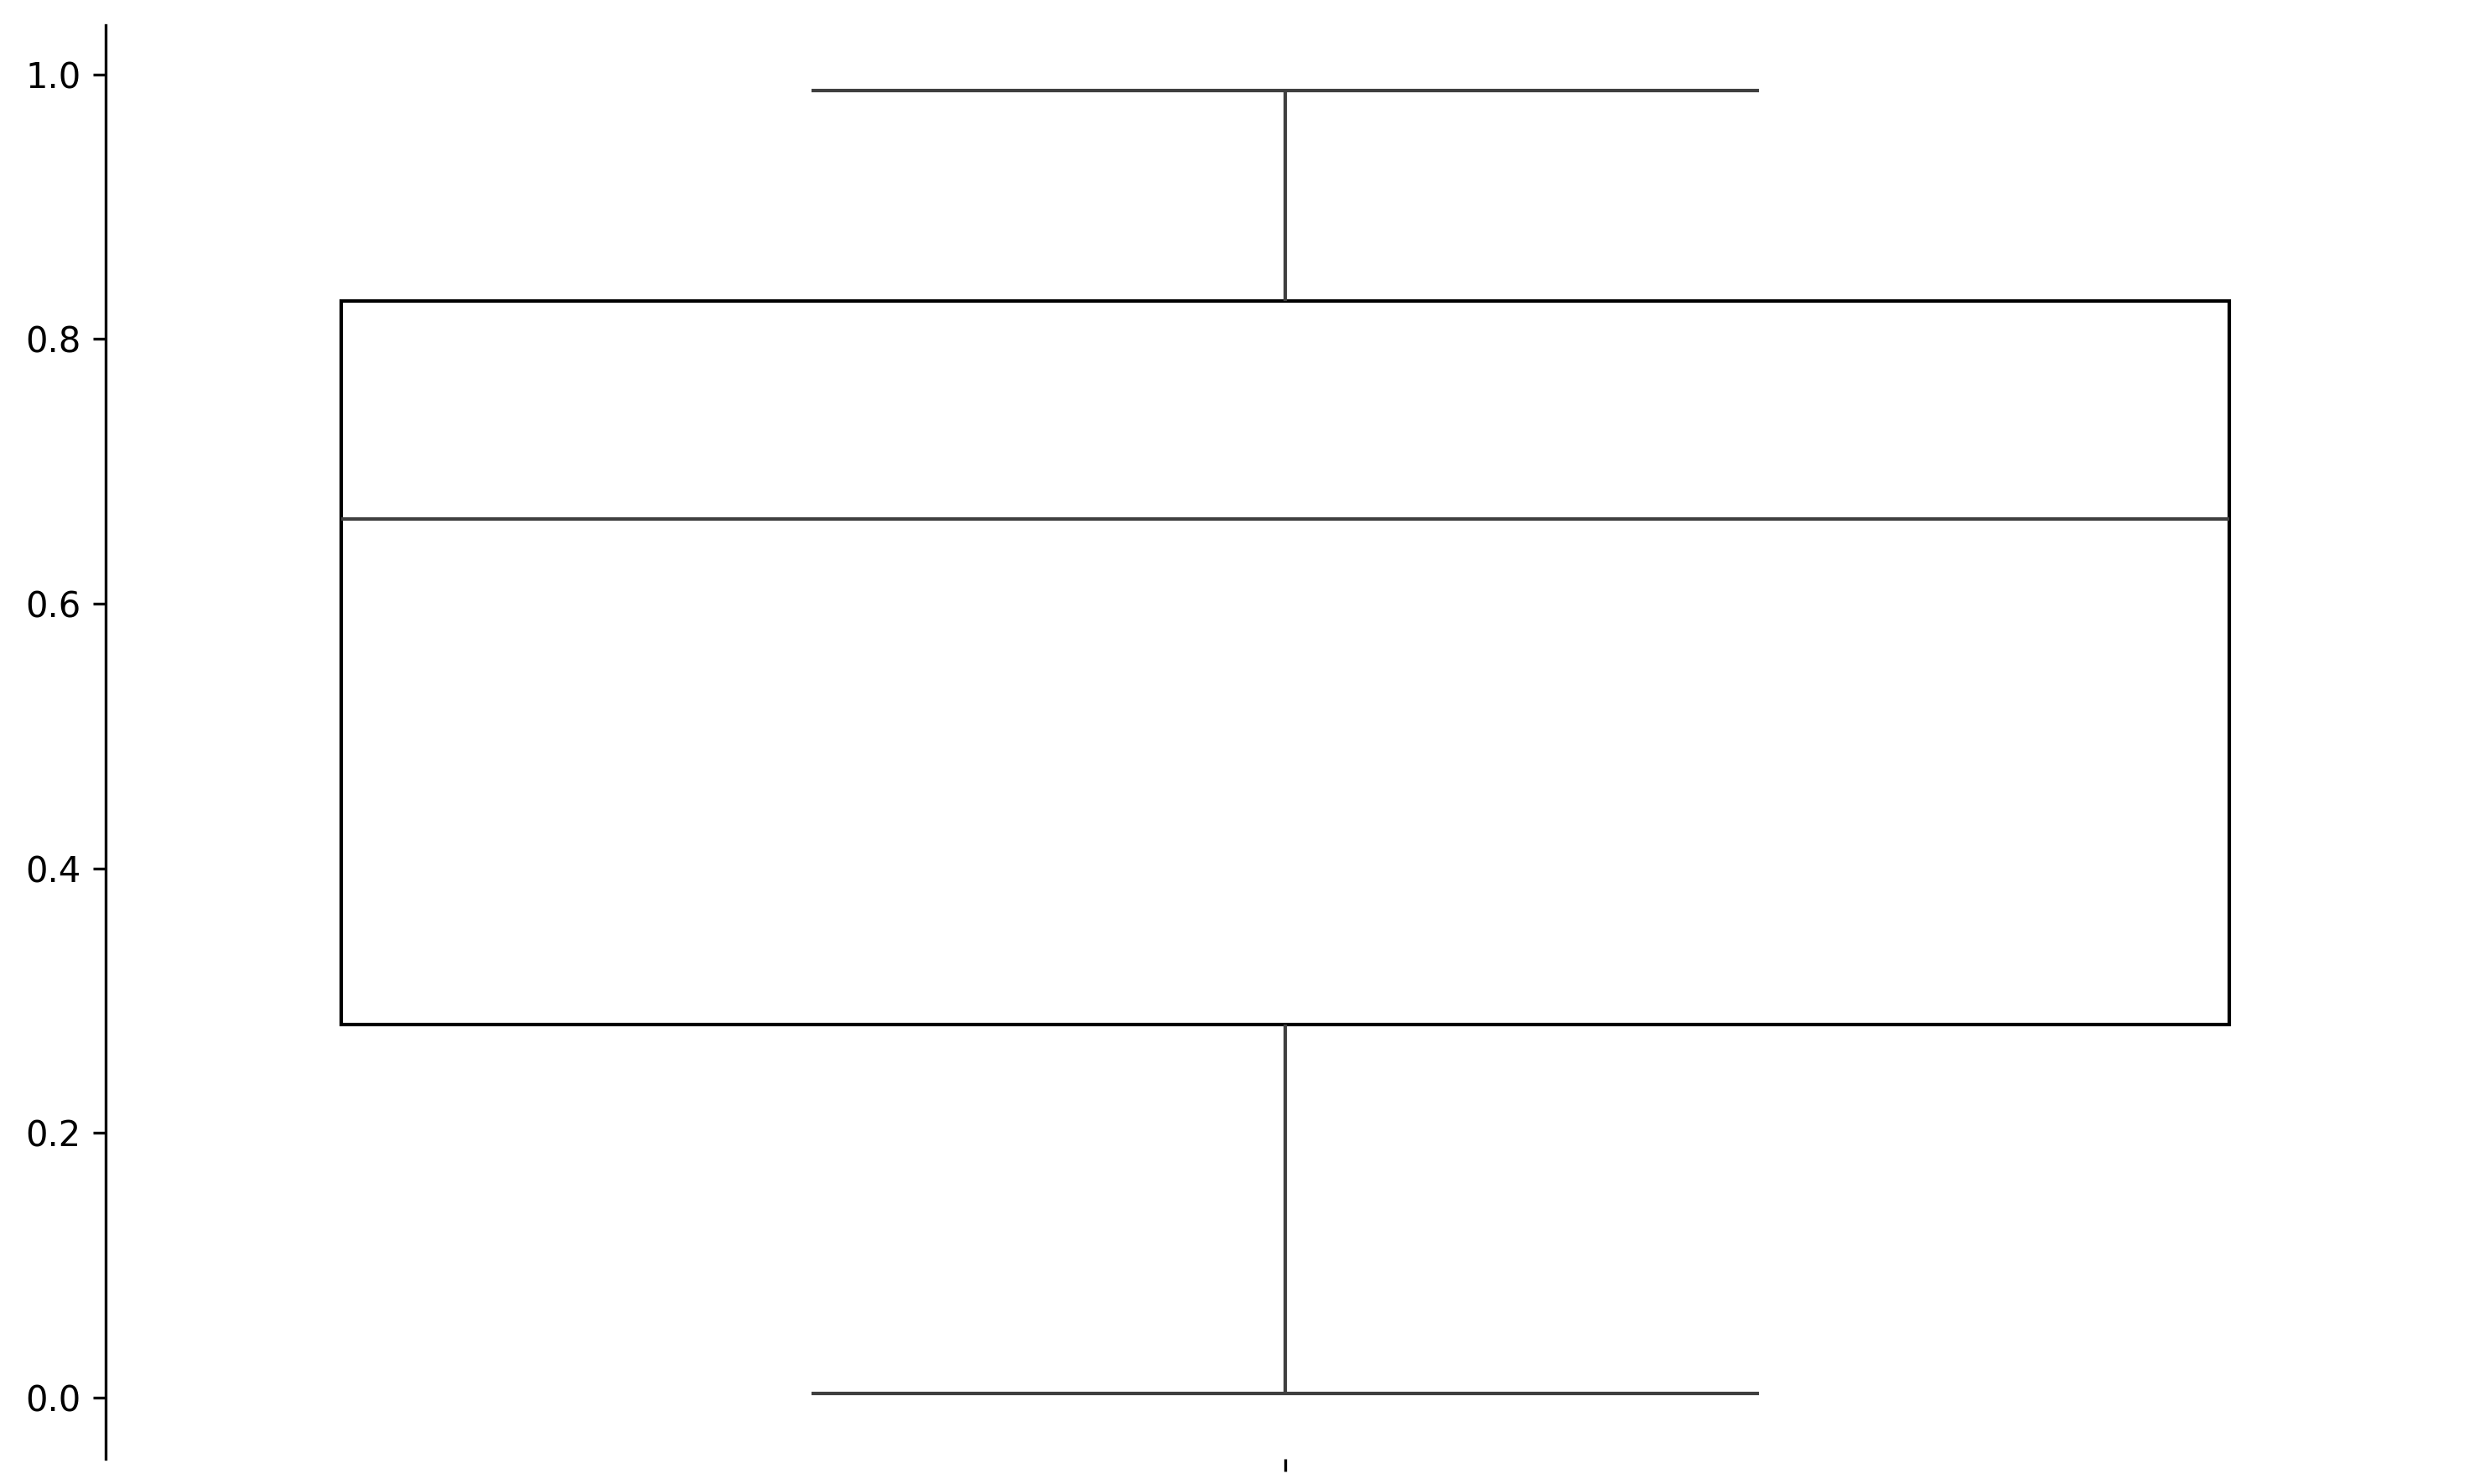
\includegraphics[width=1\linewidth]{figuras/quartis_controle_jus_sobre_gov}
    \label{fig:quartis_controle_jus_sobre_gov}
    \footnotesize{Fonte: elaboração própia baseada em \cite{jus_constraints_on_gov}.}
\end{figure}

A figura \ref{fig:quartis_controle_jus_sobre_gov}, que mostra a distribuição do índice de controle judicial sobre o Poder Executivo, ilustra que no ano de 2024 teve um valor mínimo de 0,003 e um máximo de 0,988. A média dos dados foi de 0,664. Além disso, 25\% dos valores ficaram abaixo de 0,282 (1º quartil), enquanto 75\% dos valores foram inferiores a 0,829 (3º quartil).

A figura \ref{fig:judicial-corruption-score} mostra os índices globais de corrupção judiciária.

\begin{figure}[H]
	\centering
	\caption{Pontuação de corrupção judicial no mundo em 2024}
	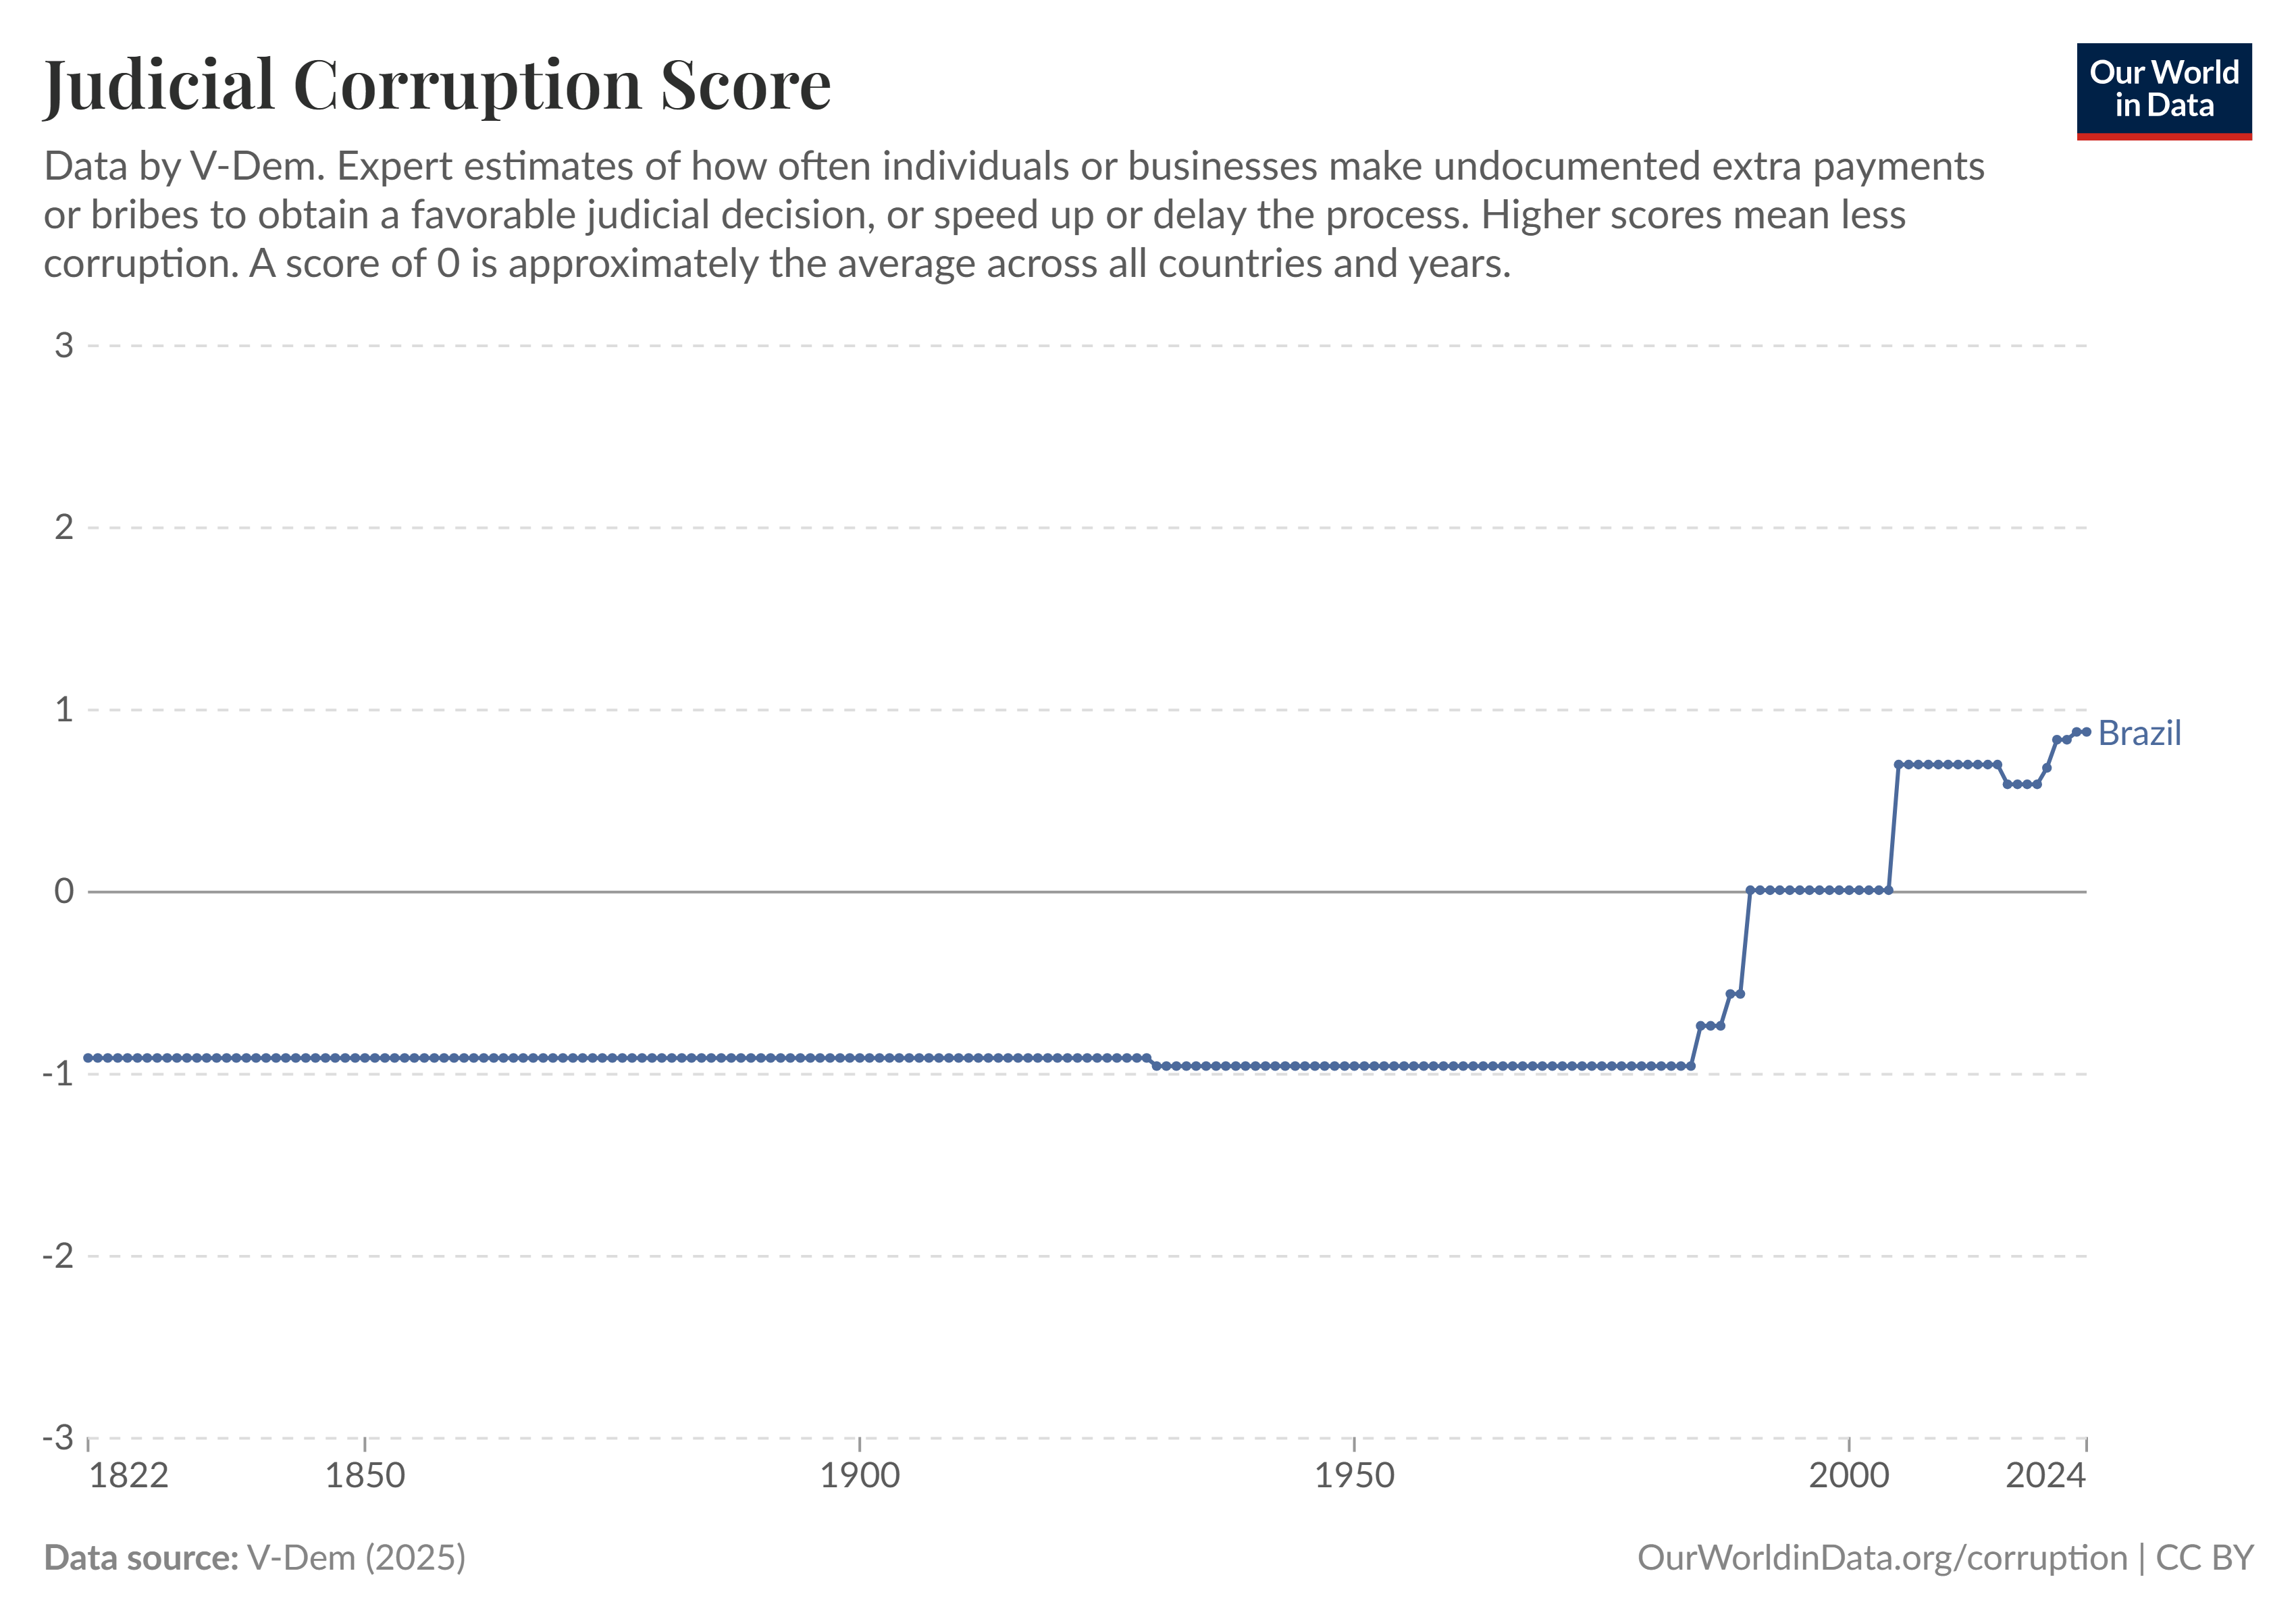
\includegraphics[width=1\linewidth]{figuras/judicial-corruption-score}
	\label{fig:judicial-corruption-score}
	\footnotesize{Fonte: \cite{judicial-corruption-score}.}
\end{figure}

Nota-se que uma quantidade grande de países tem alta corrupção judiciária. A figura \ref{fig:judicial-corruption-score} complementa a anterior ao especificar a situação histórica do Brasil (desde 1822 até 2024).

A figura \ref{fig:judicial-corruption-score-brazil} mostra como o Brasil melhorou o aspecto da corrupção judiciária. 

\begin{figure}[H]
    \centering
    \caption{Pontuação de corrupção judicial no Brasil (1822-2024)}
    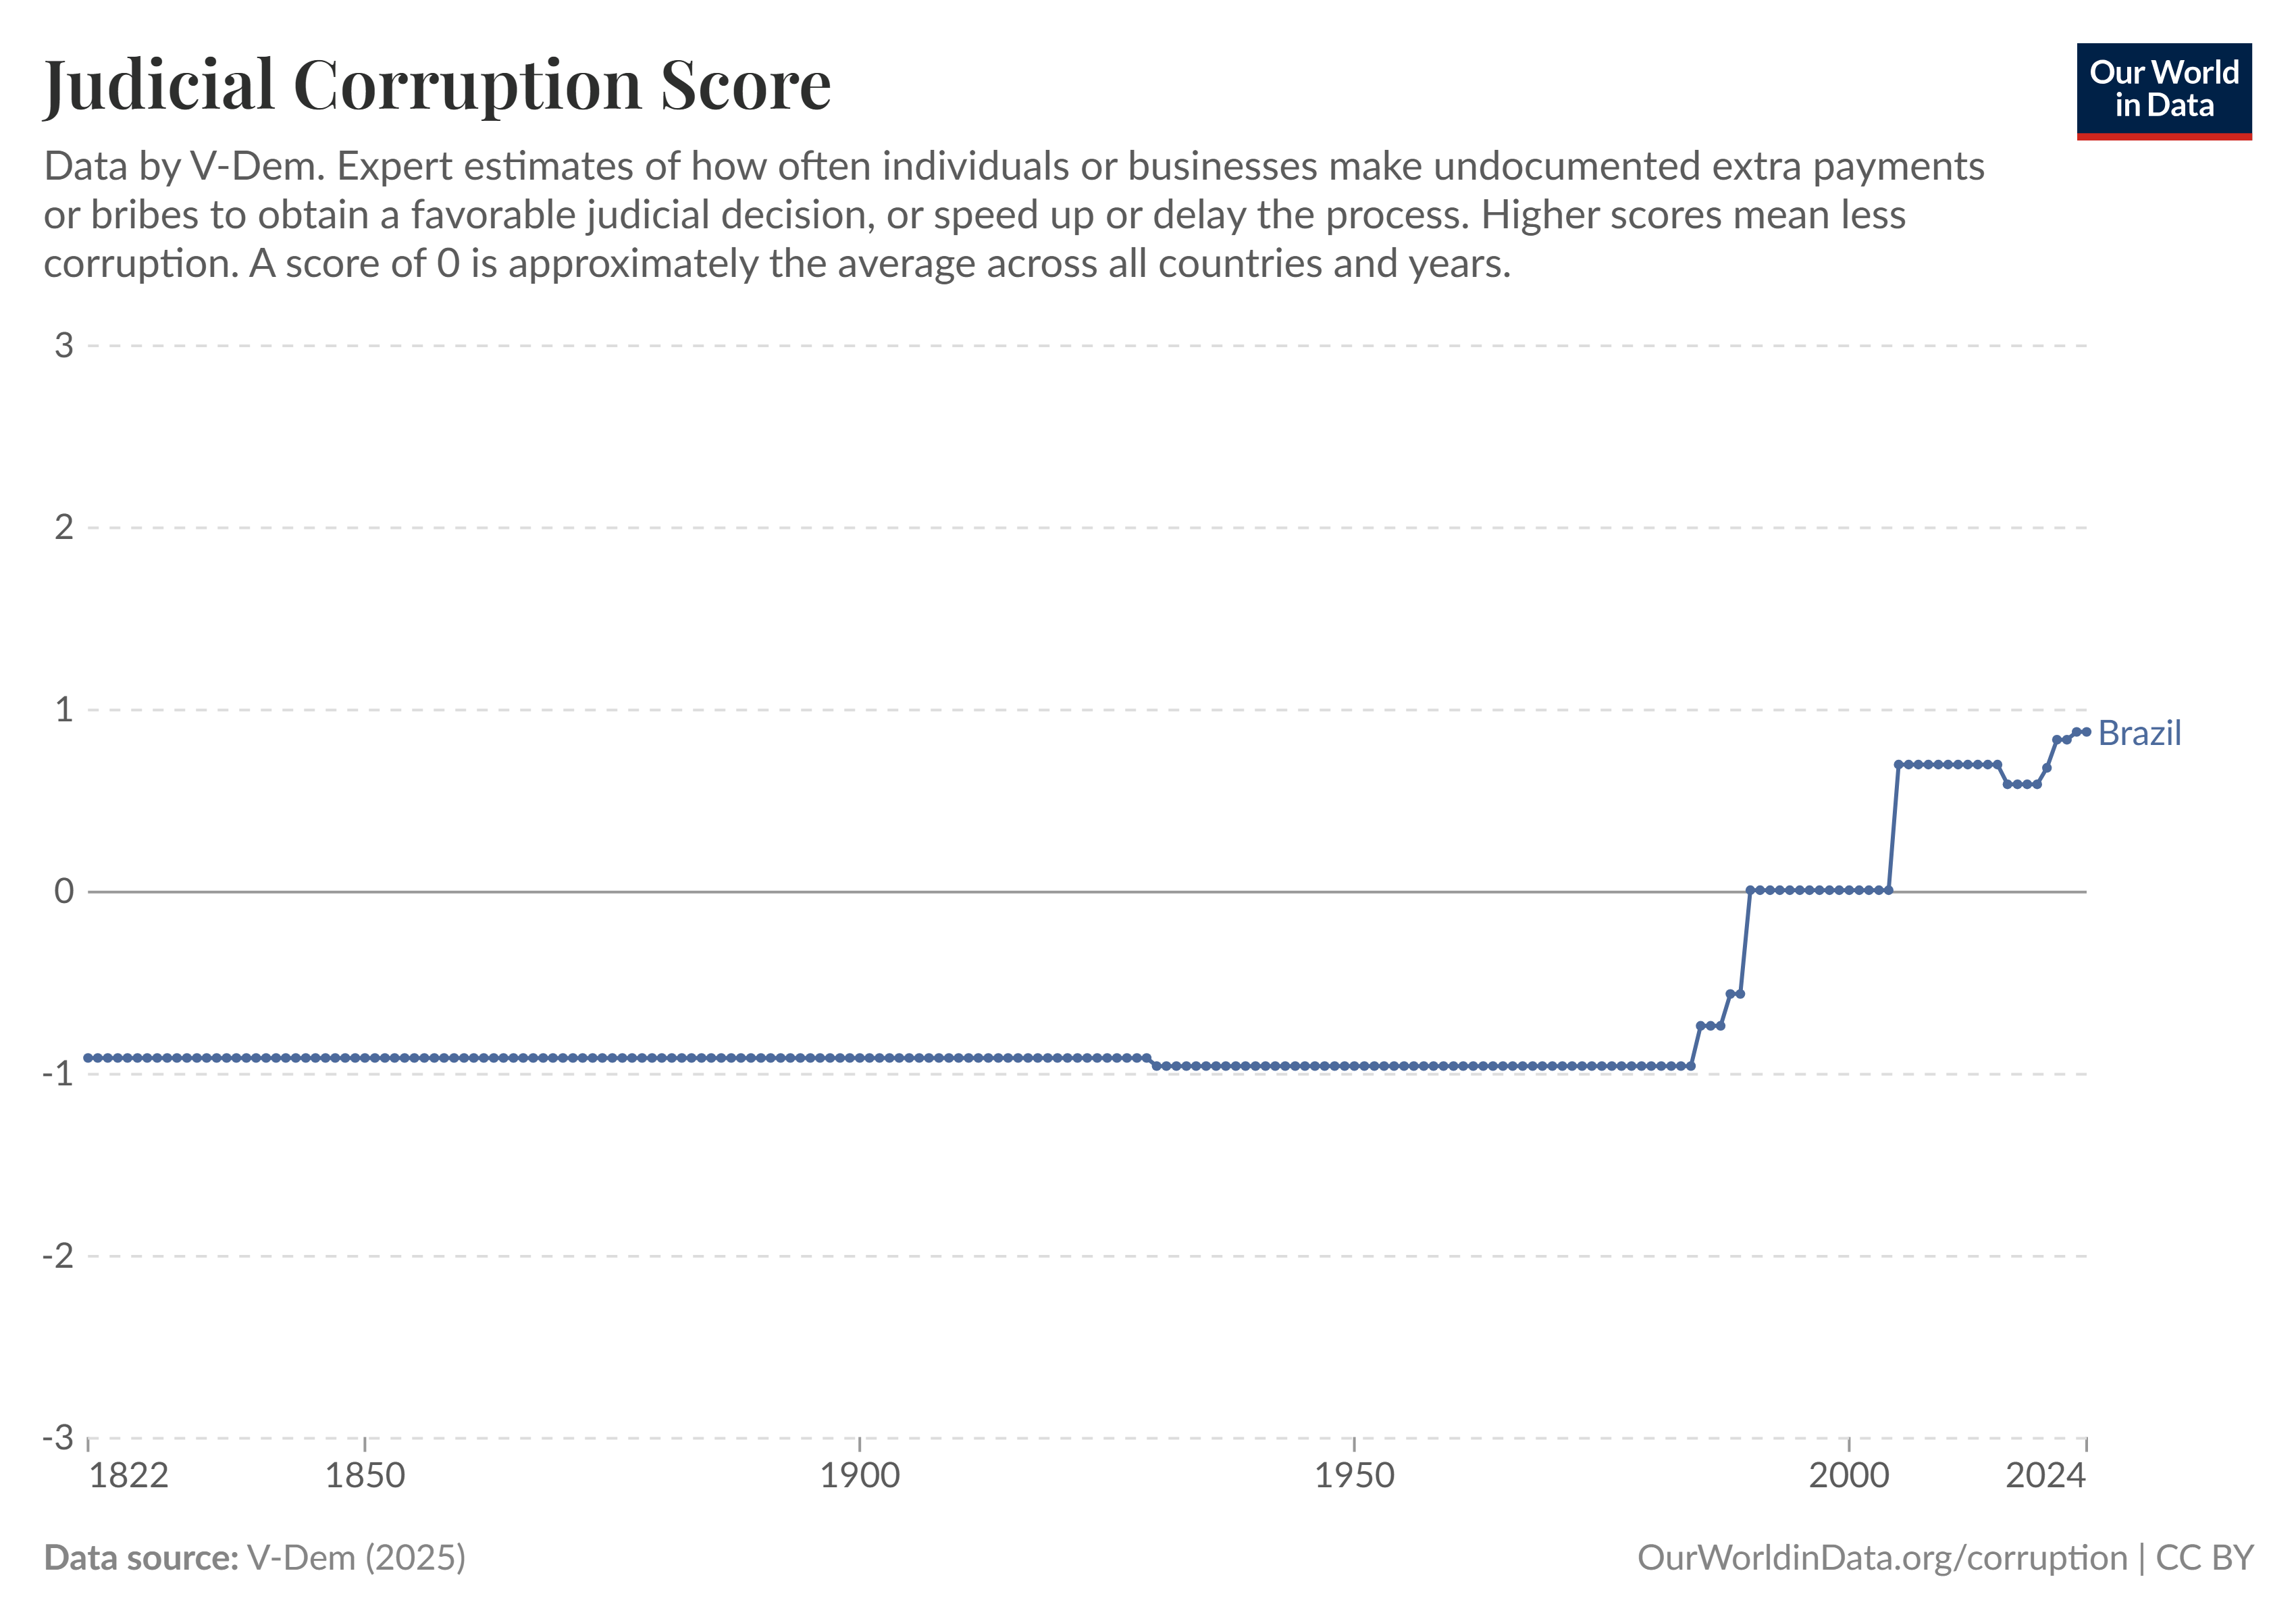
\includegraphics[width=1\linewidth]{figuras/judicial-corruption-score-brazil}
    \label{fig:judicial-corruption-score-brazil}
    \footnotesize{Fonte: \cite{judicial-corruption-score}.}
\end{figure}

Durante décadas, o Brasil ficou na faixa -1, alcançando 0 até 0,88. A atual pontuação do Brasil não está entre as melhores, pois ainda há as pontuações 2 e 3. No entanto, como a média mundial foi 0,249, o Brasil está acima da média mundial, porém o país foi superado por 66 países, cujas pontuações superaram 0,88. A quantidade de países que atingiu, no mínimo, 1 foi 29,84\%; no tocante a pontuação 2, foi 12\%; e por fim, 3 foi 3\% e nenhum atingiu 4 (valor máximo).

De maneira complementar, a figura \ref{fig:quartis_corrupcao_judiciaria} contém o gráfico de caixa da pontuação de corrupção judicial.

\begin{figure}[H]
    \centering
    \caption{Gráfico da caixa: corrupção judiciária}
    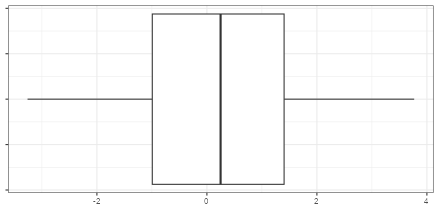
\includegraphics[width=1\linewidth]{figuras/quartis_corrupcao_judiciaria}
    \label{fig:quartis_corrupcao_judiciaria}
    \footnotesize{Fonte: elaboração própria baseada em \cite{judicial-corruption-score}.}
\end{figure}

A figura \ref{fig:quartis_corrupcao_judiciaria}, que mostra a distribuição do índice de corrupção judiciária, ilustra que no ano de 2024 teve um valor mínimo de -3,2610 e um máximo de 3,7690. A média dos dados foi de 0,2490. Além disso, 25\% dos valores ficaram abaixo de -0,9930 (1º quartil), enquanto 75\% dos valores foram inferiores a 1,4035 (3º quartil).

A figura \ref{fig:rule-of-law-index} mostra como a situação em 2024 do Estado de Direito no mundo.

\begin{figure}[H]
	\centering
	\caption{Estado de Direito no mundo em 2024}
	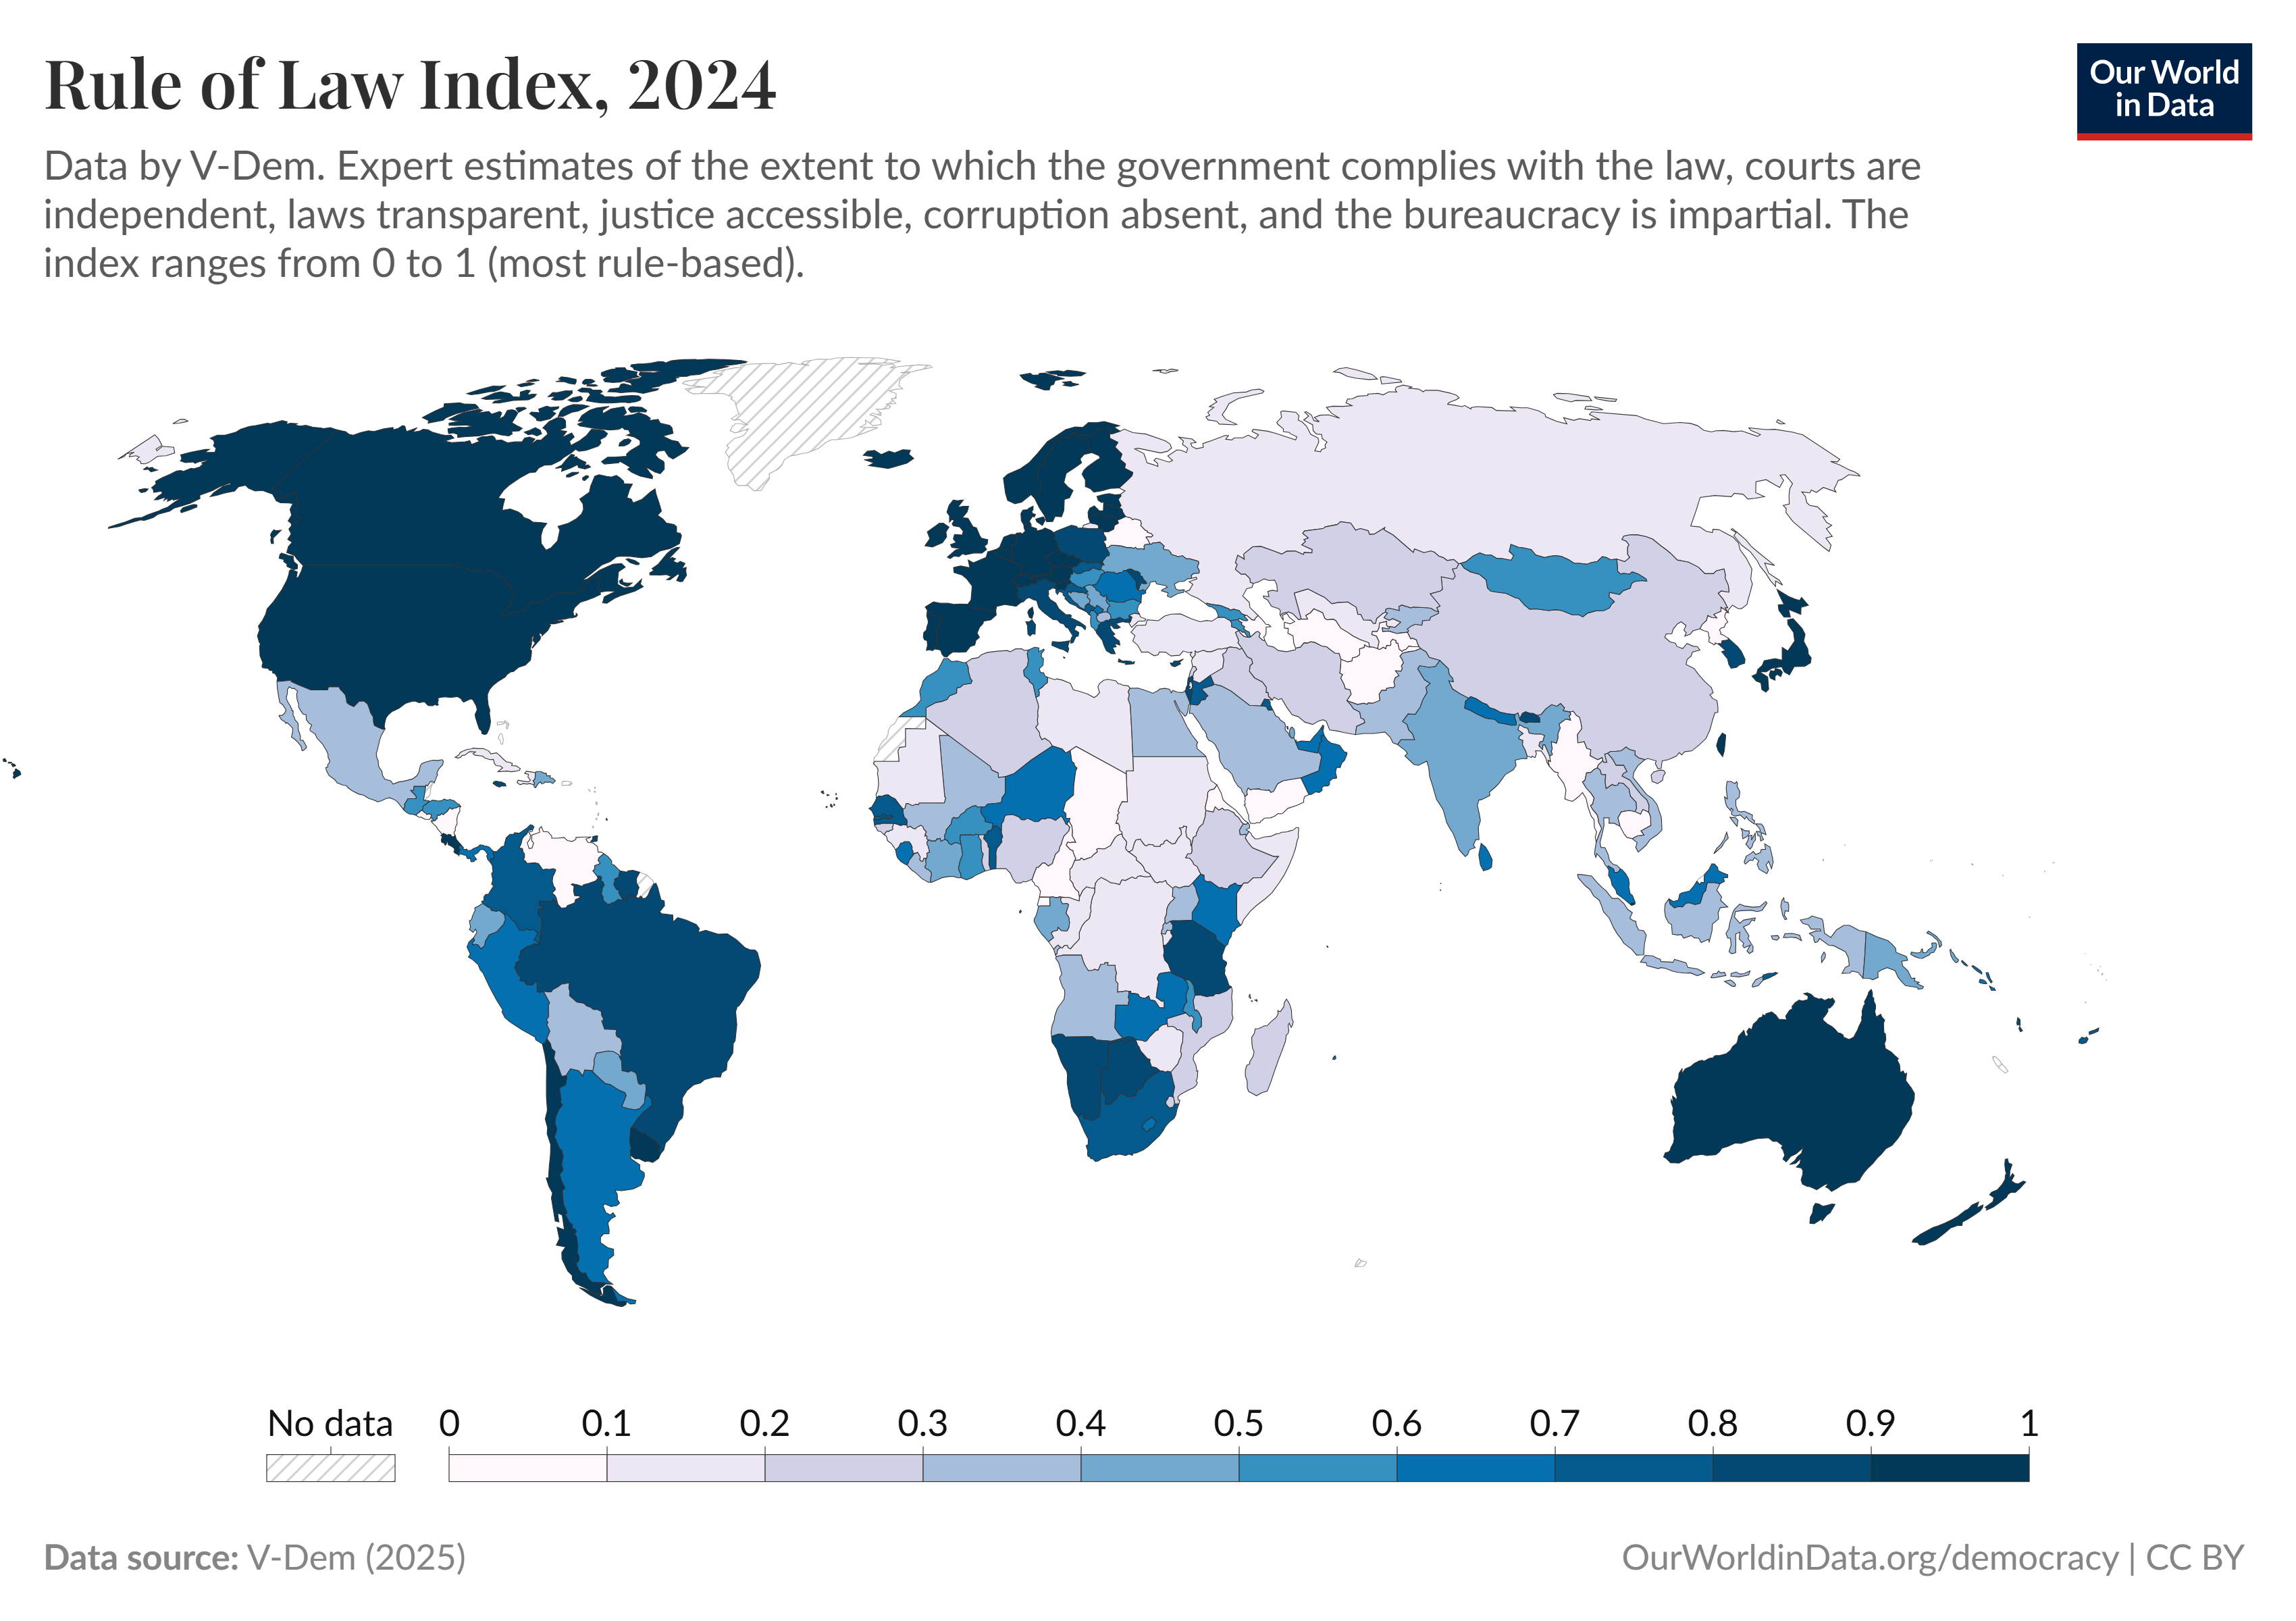
\includegraphics[width=1\linewidth]{figuras/rule-of-law-index}
	\label{fig:rule-of-law-index}
	\footnotesize{Fonte: \cite{rule-of-law-index}.}
\end{figure}

Nota-se como a instituição do Estado de Direito é muito fraco ou inexistente em muitos países do globo. De forma complementar a figura anterior, a figura \ref{fig:rule-of-law-index-brazil} mostra à situação histórica do Estado de Direito no Brasil (desde 1822 até 2024)

\begin{figure}[H]
	\centering
	\caption{Estado de Direito no Brasil (1822-2024)}
	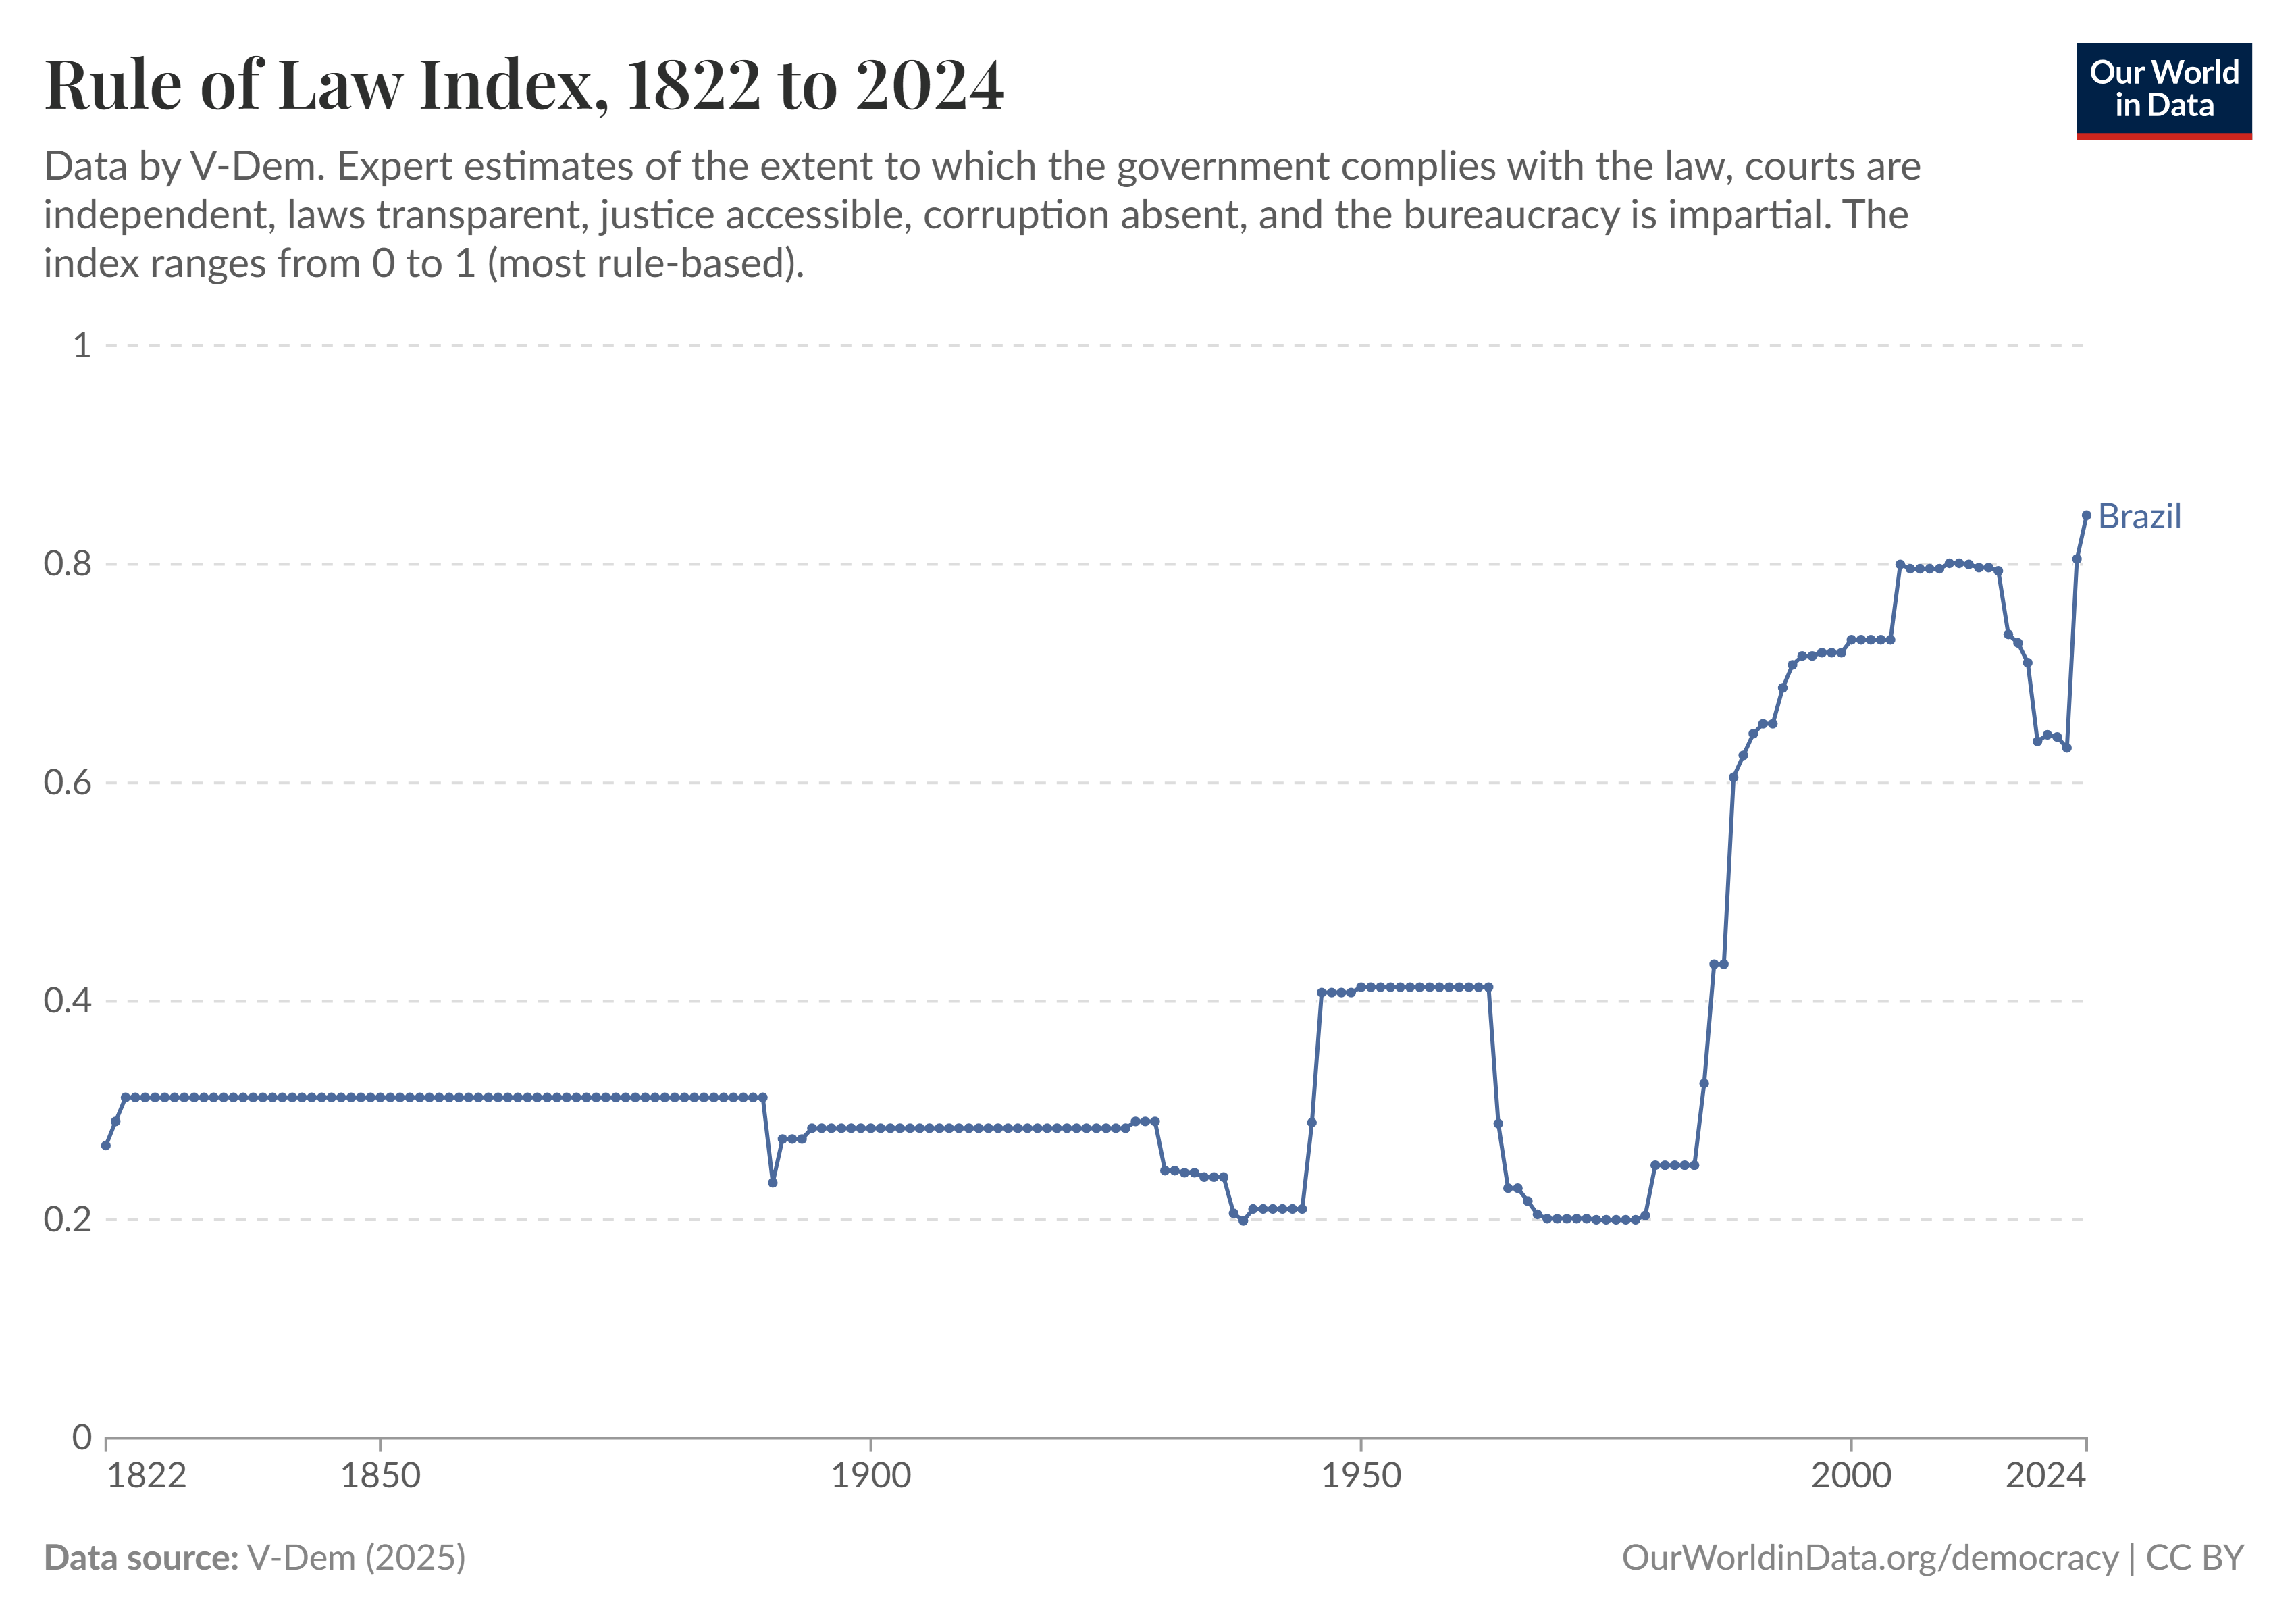
\includegraphics[width=1\linewidth]{figuras/rule-of-law-index-brazil}
	\label{fig:rule-of-law-index-brazil}
	\footnotesize{Fonte: \cite{rule-of-law-index}.}
\end{figure}

Nota-se como o Brasil evoluiu no aspecto do Estado de Direito. Durante mais de 100 anos (1822 até quase 1950), o Brasil ficou na faixa baixa 0,2-0,4, no entanto, atingiu o valor de 0,8 em 2023 e 0,84 em 2024 via políticas públicas que almejaram esse crescimento.

A figura \ref{fig:quartis_estado_direito} contém um gráfico de caixa.

\begin{figure}[H]
	\centering
	\caption{Gráfico da caixa: Estado de Direito}
	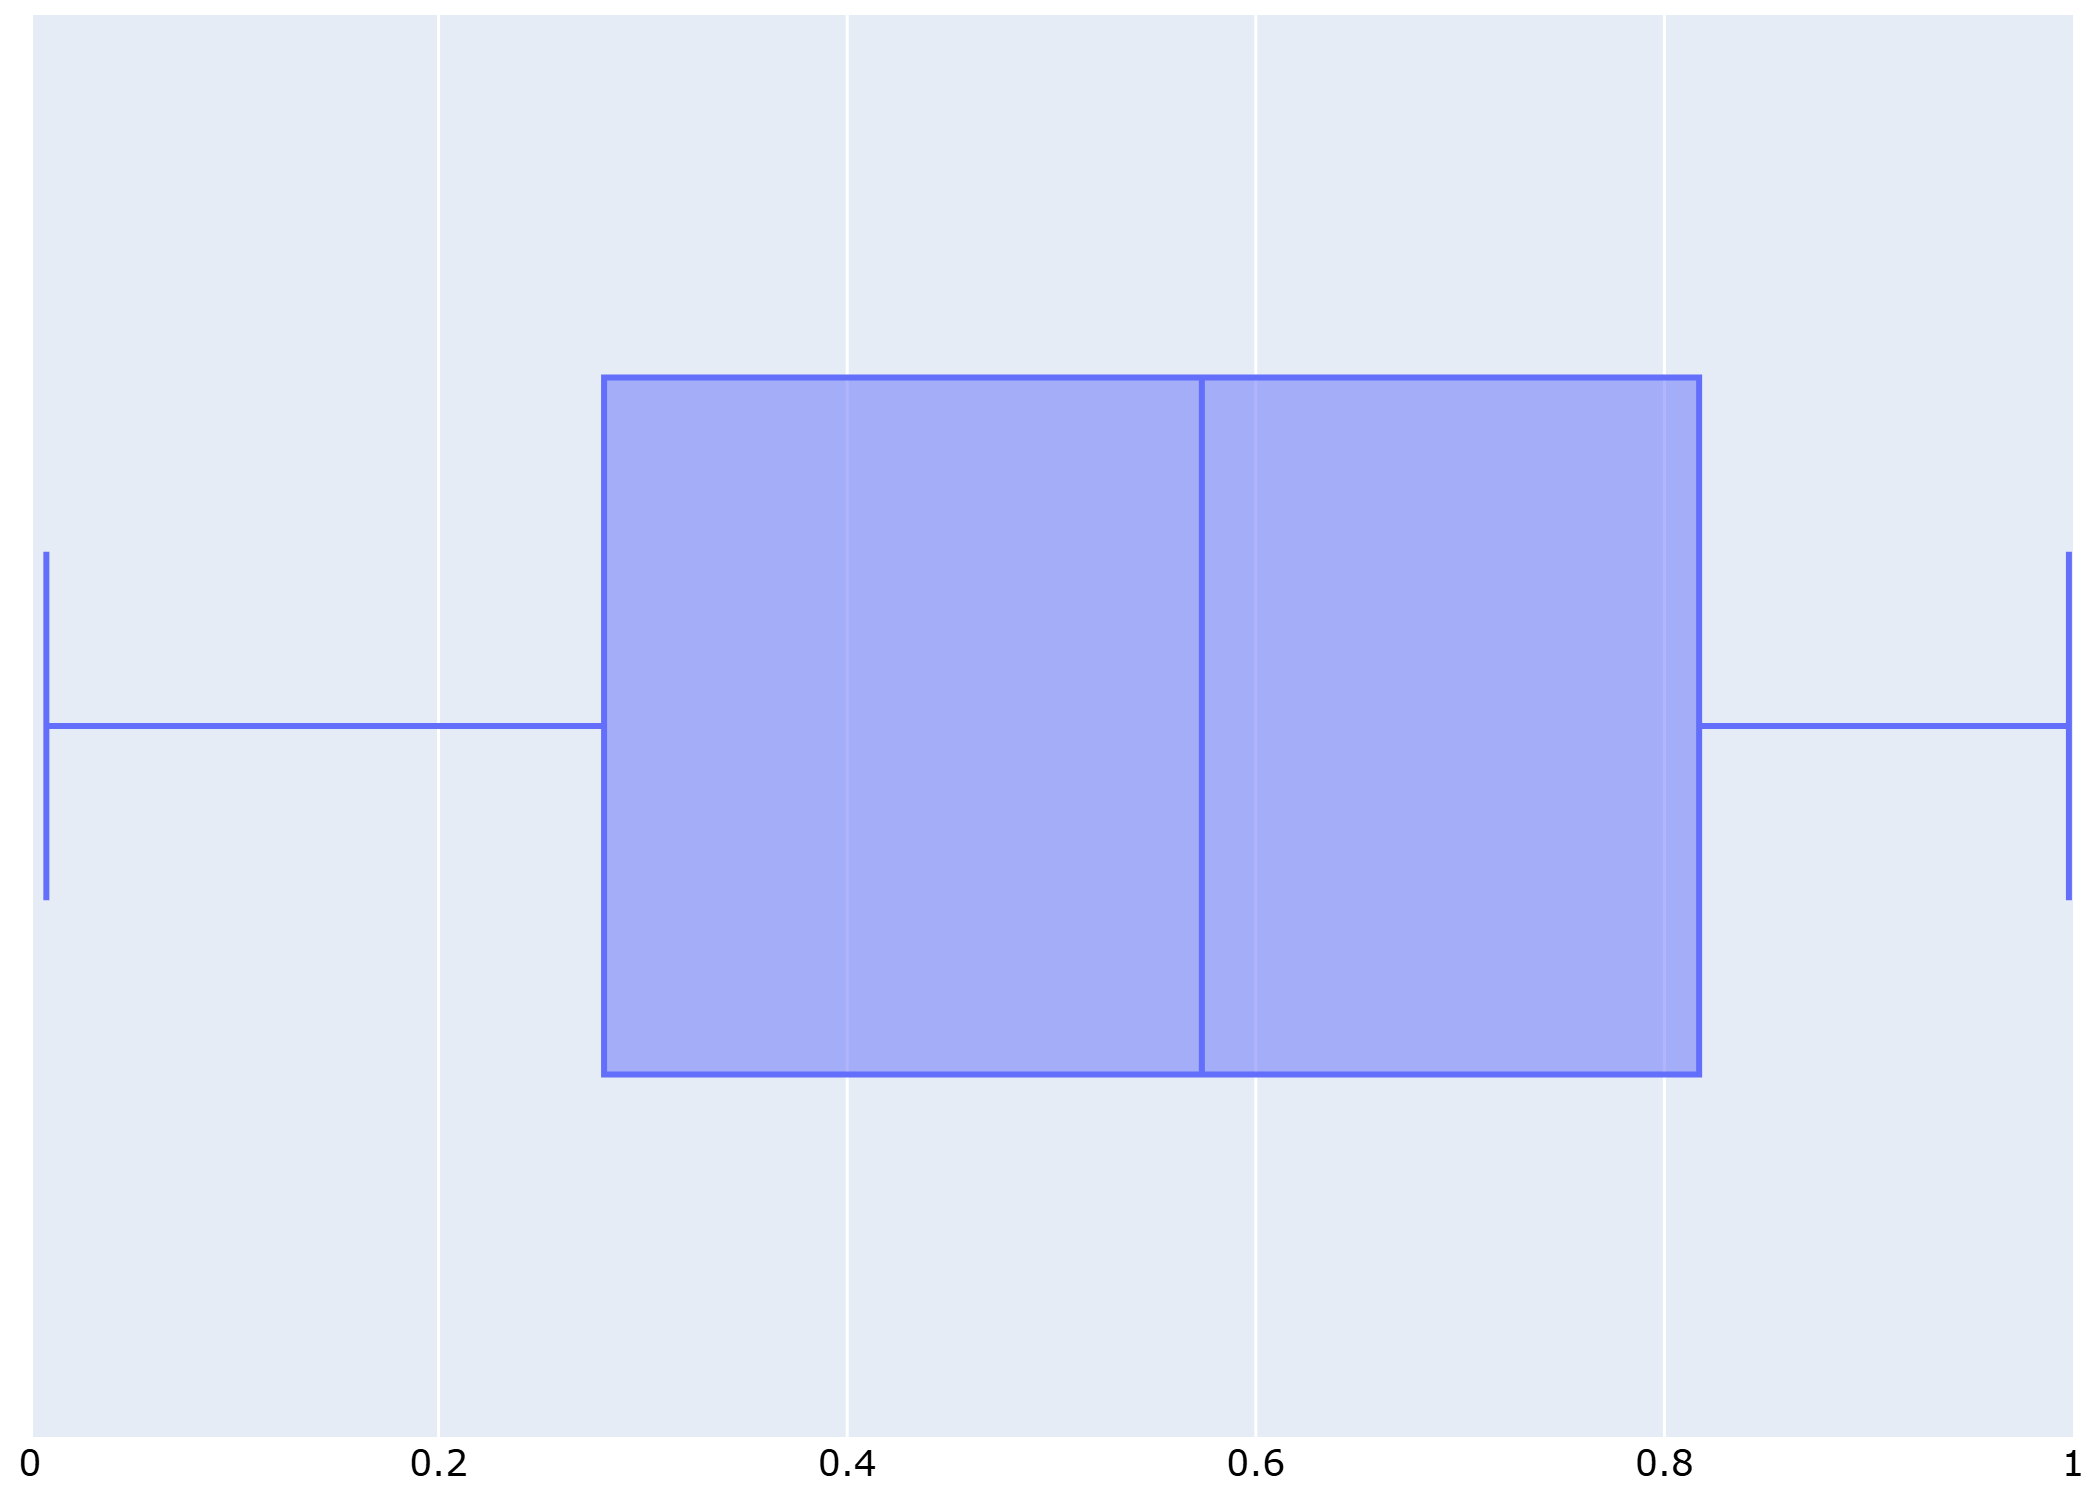
\includegraphics[width=1\linewidth]{figuras/quartis_estado_direito}
	\label{fig:quartis_estado_direito}
	\footnotesize{Fonte: elaboração própria baseada em \cite{rule-of-law-index}.}
\end{figure}

A figura \ref{fig:quartis_estado_direito}, que mostra a distribuição do índice de corrupção judiciária, ilustra que no ano de 2024 teve um valor mínimo de 0,008 e um máximo de 0,998. A média dos dados foi de 0,5736. Além disso, 25\% dos valores ficaram abaixo de 0,282 (1º quartil), enquanto 75\% dos valores foram inferiores a 0,816 (3º quartil).

Além da análise gráfica, estudou-se se há correlação entre o índice de democracia eleitoral com os índices de controle judicial sob o Poder Executivo, corrupção no Poder Judiciário, Estado de Direito e liberdades civis.

A figura \ref{fig:comparacao_democracia} contém um gráfico de barras que contêm os coeficientes de correlação das relações entre o índice de democracia eleitoral com os índices de controle judicial sob o Poder Executivo, corrupção no Poder Judiciário, Estado de Direito e liberdades civis. A referida figura tem os elementos presentes na tabela \ref{tab:itens_comparacao_democracia}.

\begin{longtable}[c]{@{}ll@{}}
	\caption{Itens da figura \ref{fig:comparacao_democracia}}
	\label{tab:itens_comparacao_democracia}\\
	\toprule
	\textbf{Item} & \textbf{Significado} \\
	\midrule
	\endfirsthead
	\toprule
	\textbf{Item} & \textbf{Significado} \\
	\midrule
	\endhead
	%
	\bottomrule
	\endfoot
	%
	\multicolumn{2}{r}{\textbf{Continua na próxima página.}} \\*
	\endfoot
	%
	\endlastfoot
	%
	C1 &
	\begin{tabular}[c]{@{}l@{}}Índice de Democracia Eleitoral \\ x \\ Corrupção Judicial.\end{tabular} \\ \midrule
	C2 &
	\begin{tabular}[c]{@{}l@{}}Índice de Democracia Eleitoral \\ x \\ Índice de Controle Judicial sob o Poder Executivo.\end{tabular} \\ \midrule
	C3 &
	\begin{tabular}[c]{@{}l@{}}Índice de Democracia Eleitoral \\ x \\ Índice de Liberdade Civil.\end{tabular} \\ \midrule
	C4 &
	\begin{tabular}[c]{@{}l@{}}Índice de Democracia Eleitoral \\ x \\ Índice de Estado de Direito.\end{tabular} \\* \bottomrule
	\footnotesize{Fonte: elaboração própria baseada em \cite{rule-of-law-index}, \cite{jus_constraints_on_gov}, \cite{judicial-corruption-score} e \cite{human-rights-index-vdem}.}
\end{longtable}

Da tabela \ref{tab:itens_comparacao_democracia}, serão usados os significados para poder interpretar os itens da figura \ref{fig:comparacao_democracia}.

\begin{figure}[H]
	\centering
	\caption{Coeficiente de correlação: índice de democracia eleitoral x índices de controle judicial sob o Poder Executivo, corrupção no Poder Judiciário, Estado de Direito e liberdades civis}
	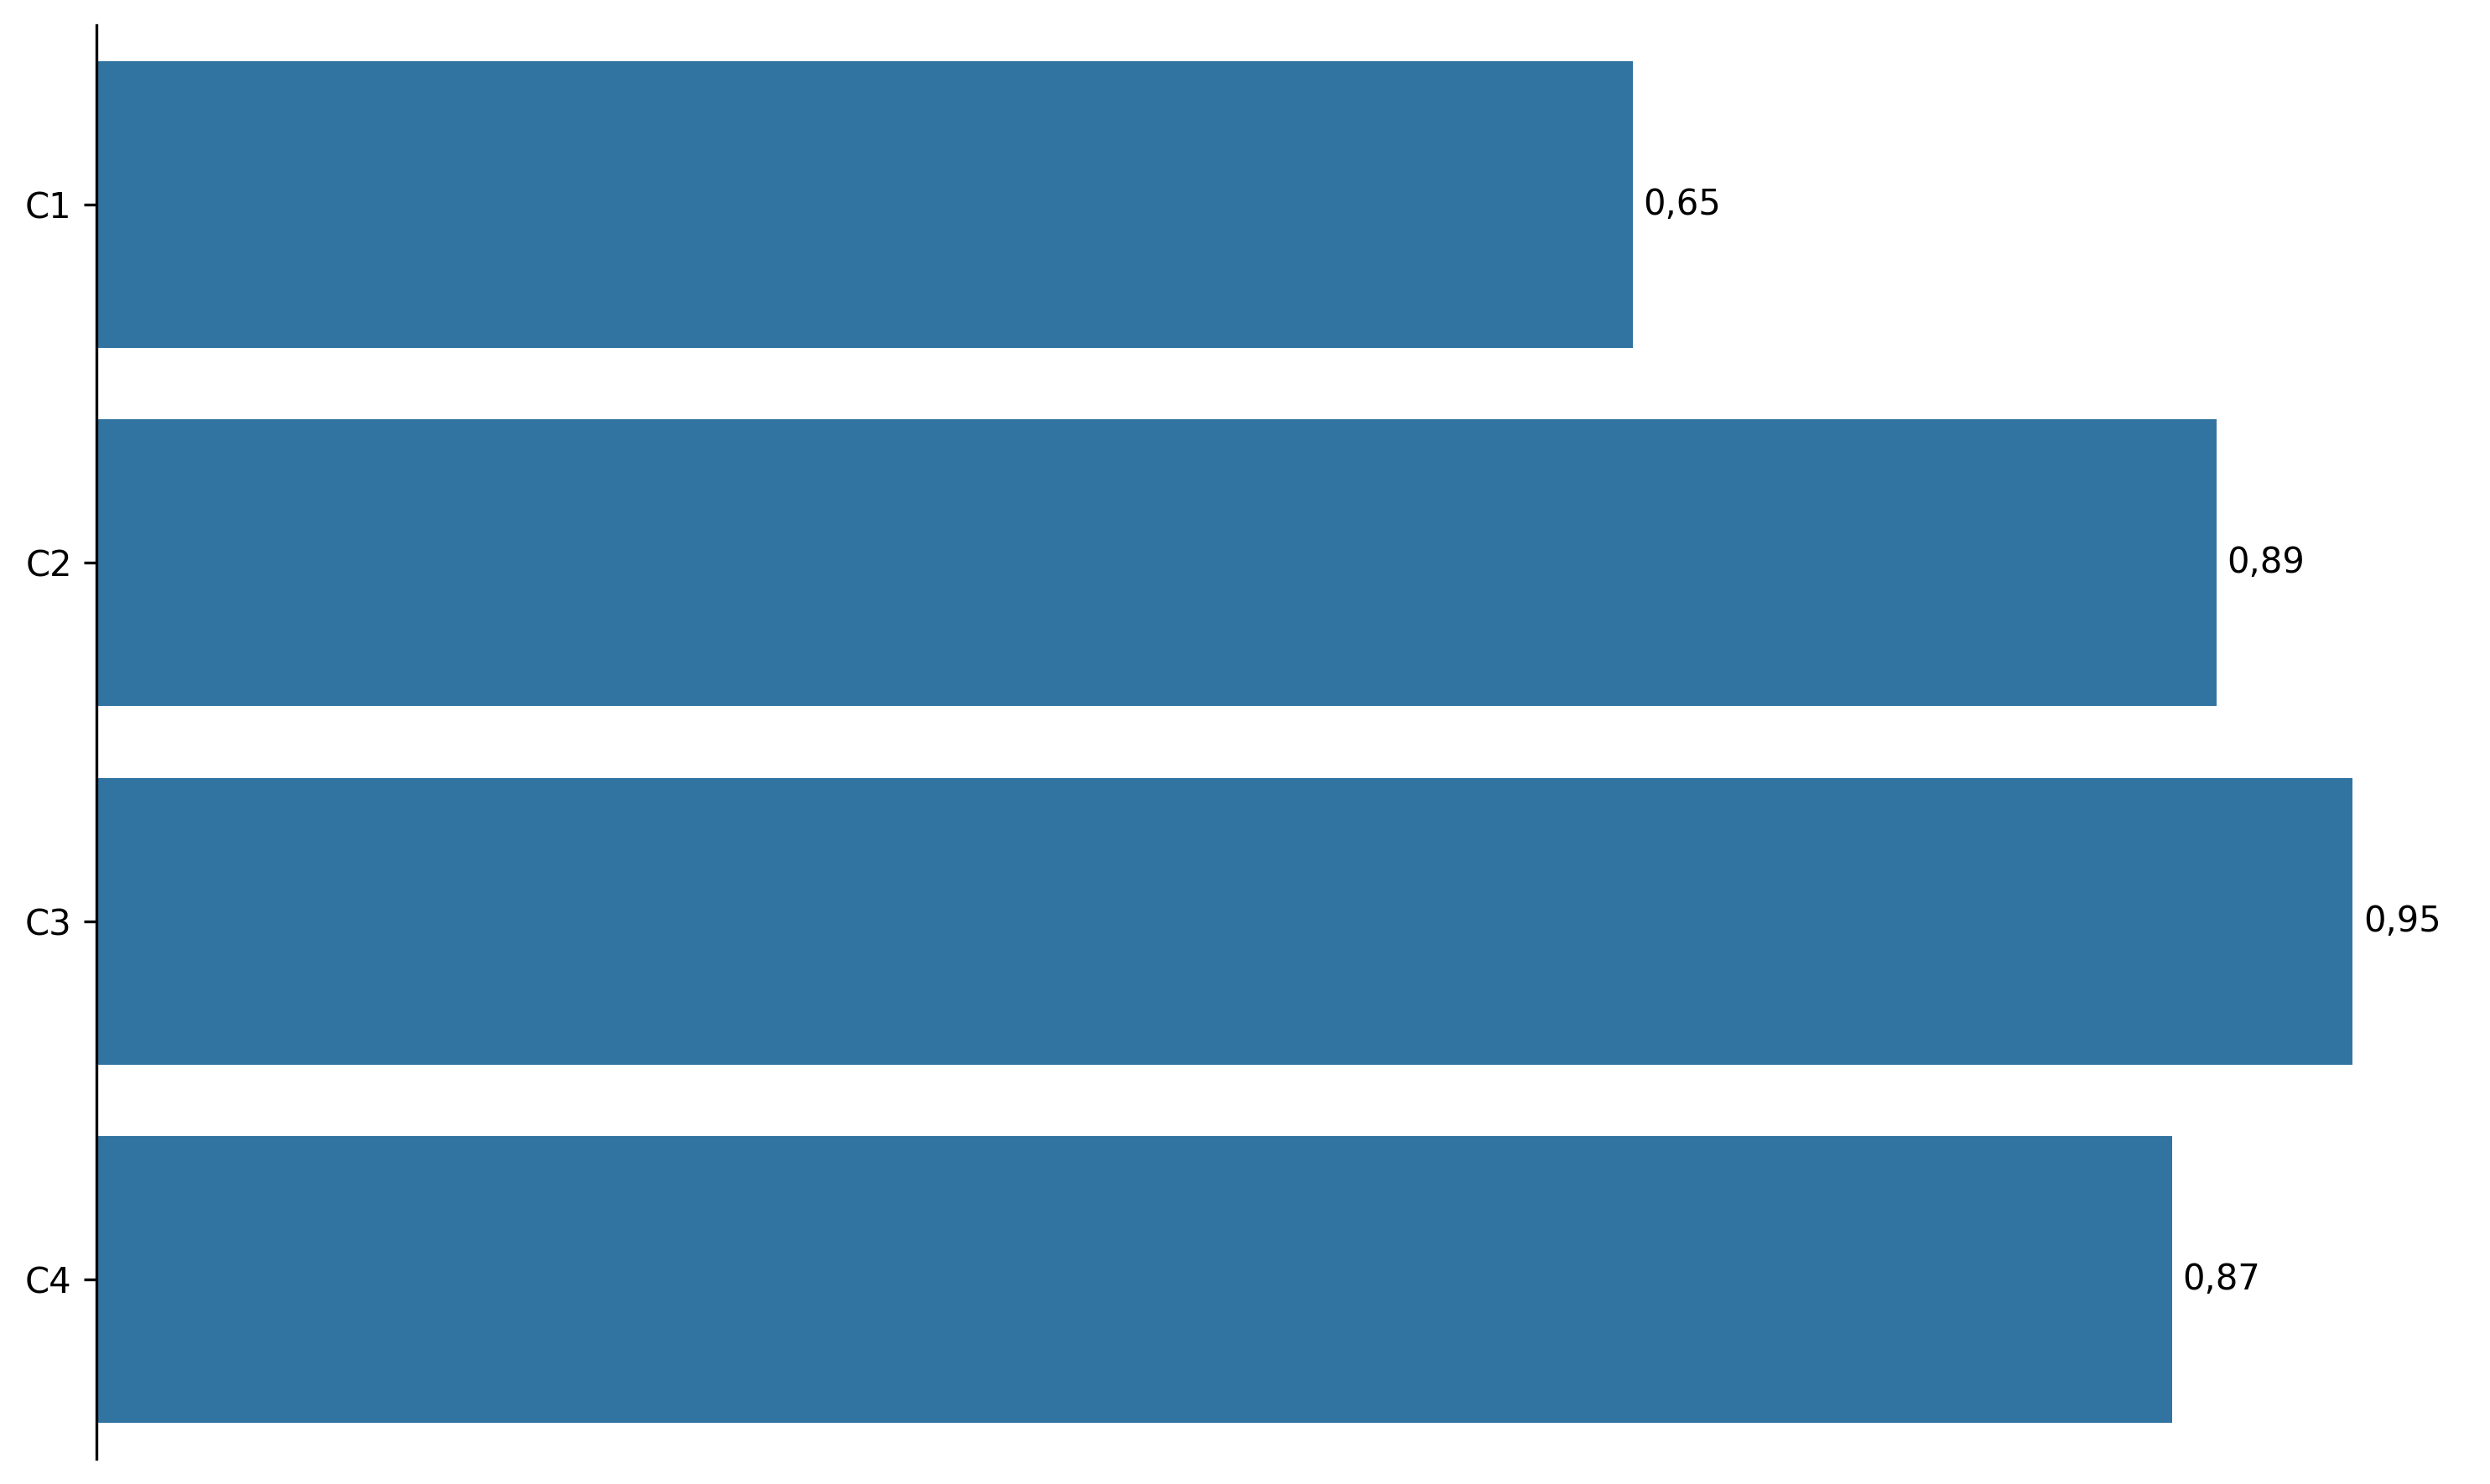
\includegraphics[width=1\linewidth]{figuras/comparacao_democracia}
	\label{fig:comparacao_democracia}
	\footnotesize{Fonte: elaboração própria baseada em \cite{rule-of-law-index}, \cite{jus_constraints_on_gov}, \cite{judicial-corruption-score} e \cite{human-rights-index-vdem}.}
\end{figure}

Nota-se da figura \ref{fig:comparacao_democracia} que a relação índice de democracia eleitoral x índice de corrupção judiciária tem uma correlação positiva média, enquanto as relações dos índices de controle judicial sob o Poder Executivo, liberdade civil e de Estado de Direito com o índice de democracia eleitoral tem correlações positivas fortes. Ou seja, controle judicial sob o Poder Executivo, liberdade civil e de Estado de Direito têm grande impacto na democracia. 

Considerando a análise de coeficiente de correlação anterior, destaque-se que o Brasil está em posição privilegiada, pois, se apenas 25\% dos 193 países alcançaram uma pontuação superior e metade alcançou menos que a média mundial, isso é um indicativo de que autocracias são prevalentes. \cite{nord2025democracy} informa que o Brasil, juntamente com o Equador, Lesoto e a Polônia, pararam e reverteram processos de autocratização antes da disrupção da democracia, exibindo resiliência a rupturas autocráticas.

Outros dados que reforçam a importância da democracia no Brasil foram apresentados por \cite{nord2025democracy} no relatório \textbf{Democracy Report 2025} da V-Dem relativo ao ano de 2024 na lista abaixo:

\begin{itemize}
    \item Democracias liberais representam menos de 12\% da população mundial, ou seja, menos de 900 milhões de pessoas.
    \item Democracias eleitorais representam 17\% da população mundial.
    \item 40\%  da população mundial - 3,1 bilhões de pessoas - vive em países que estão em processo de autocratização.
    \item Há mais autocracias do que democracias no mundo: 91 contra 88. Em 2023, era o contrário.
    \item O mundo tem apenas 29 democracias liberais, o que torna o regime o mesmo comum.
    \item 72\% das pessoas no mundo vivem em autocracias, percentual mais alto desde 1978.
\end{itemize}

\section{O Poder Judiciário como garantidor de direitos do Brasil}

Dados internacionais confirma a real democracia do Brasil. \cite{rule-of-law-index} mostra na figura \ref{fig:key-features-of-liberal-democracy} como os índices de uma democracia liberal no Brasil são altos.

\begin{figure}[H]
	\centering
	\caption{Característica principal de democracia eleitoral no Brasil em 2024}
	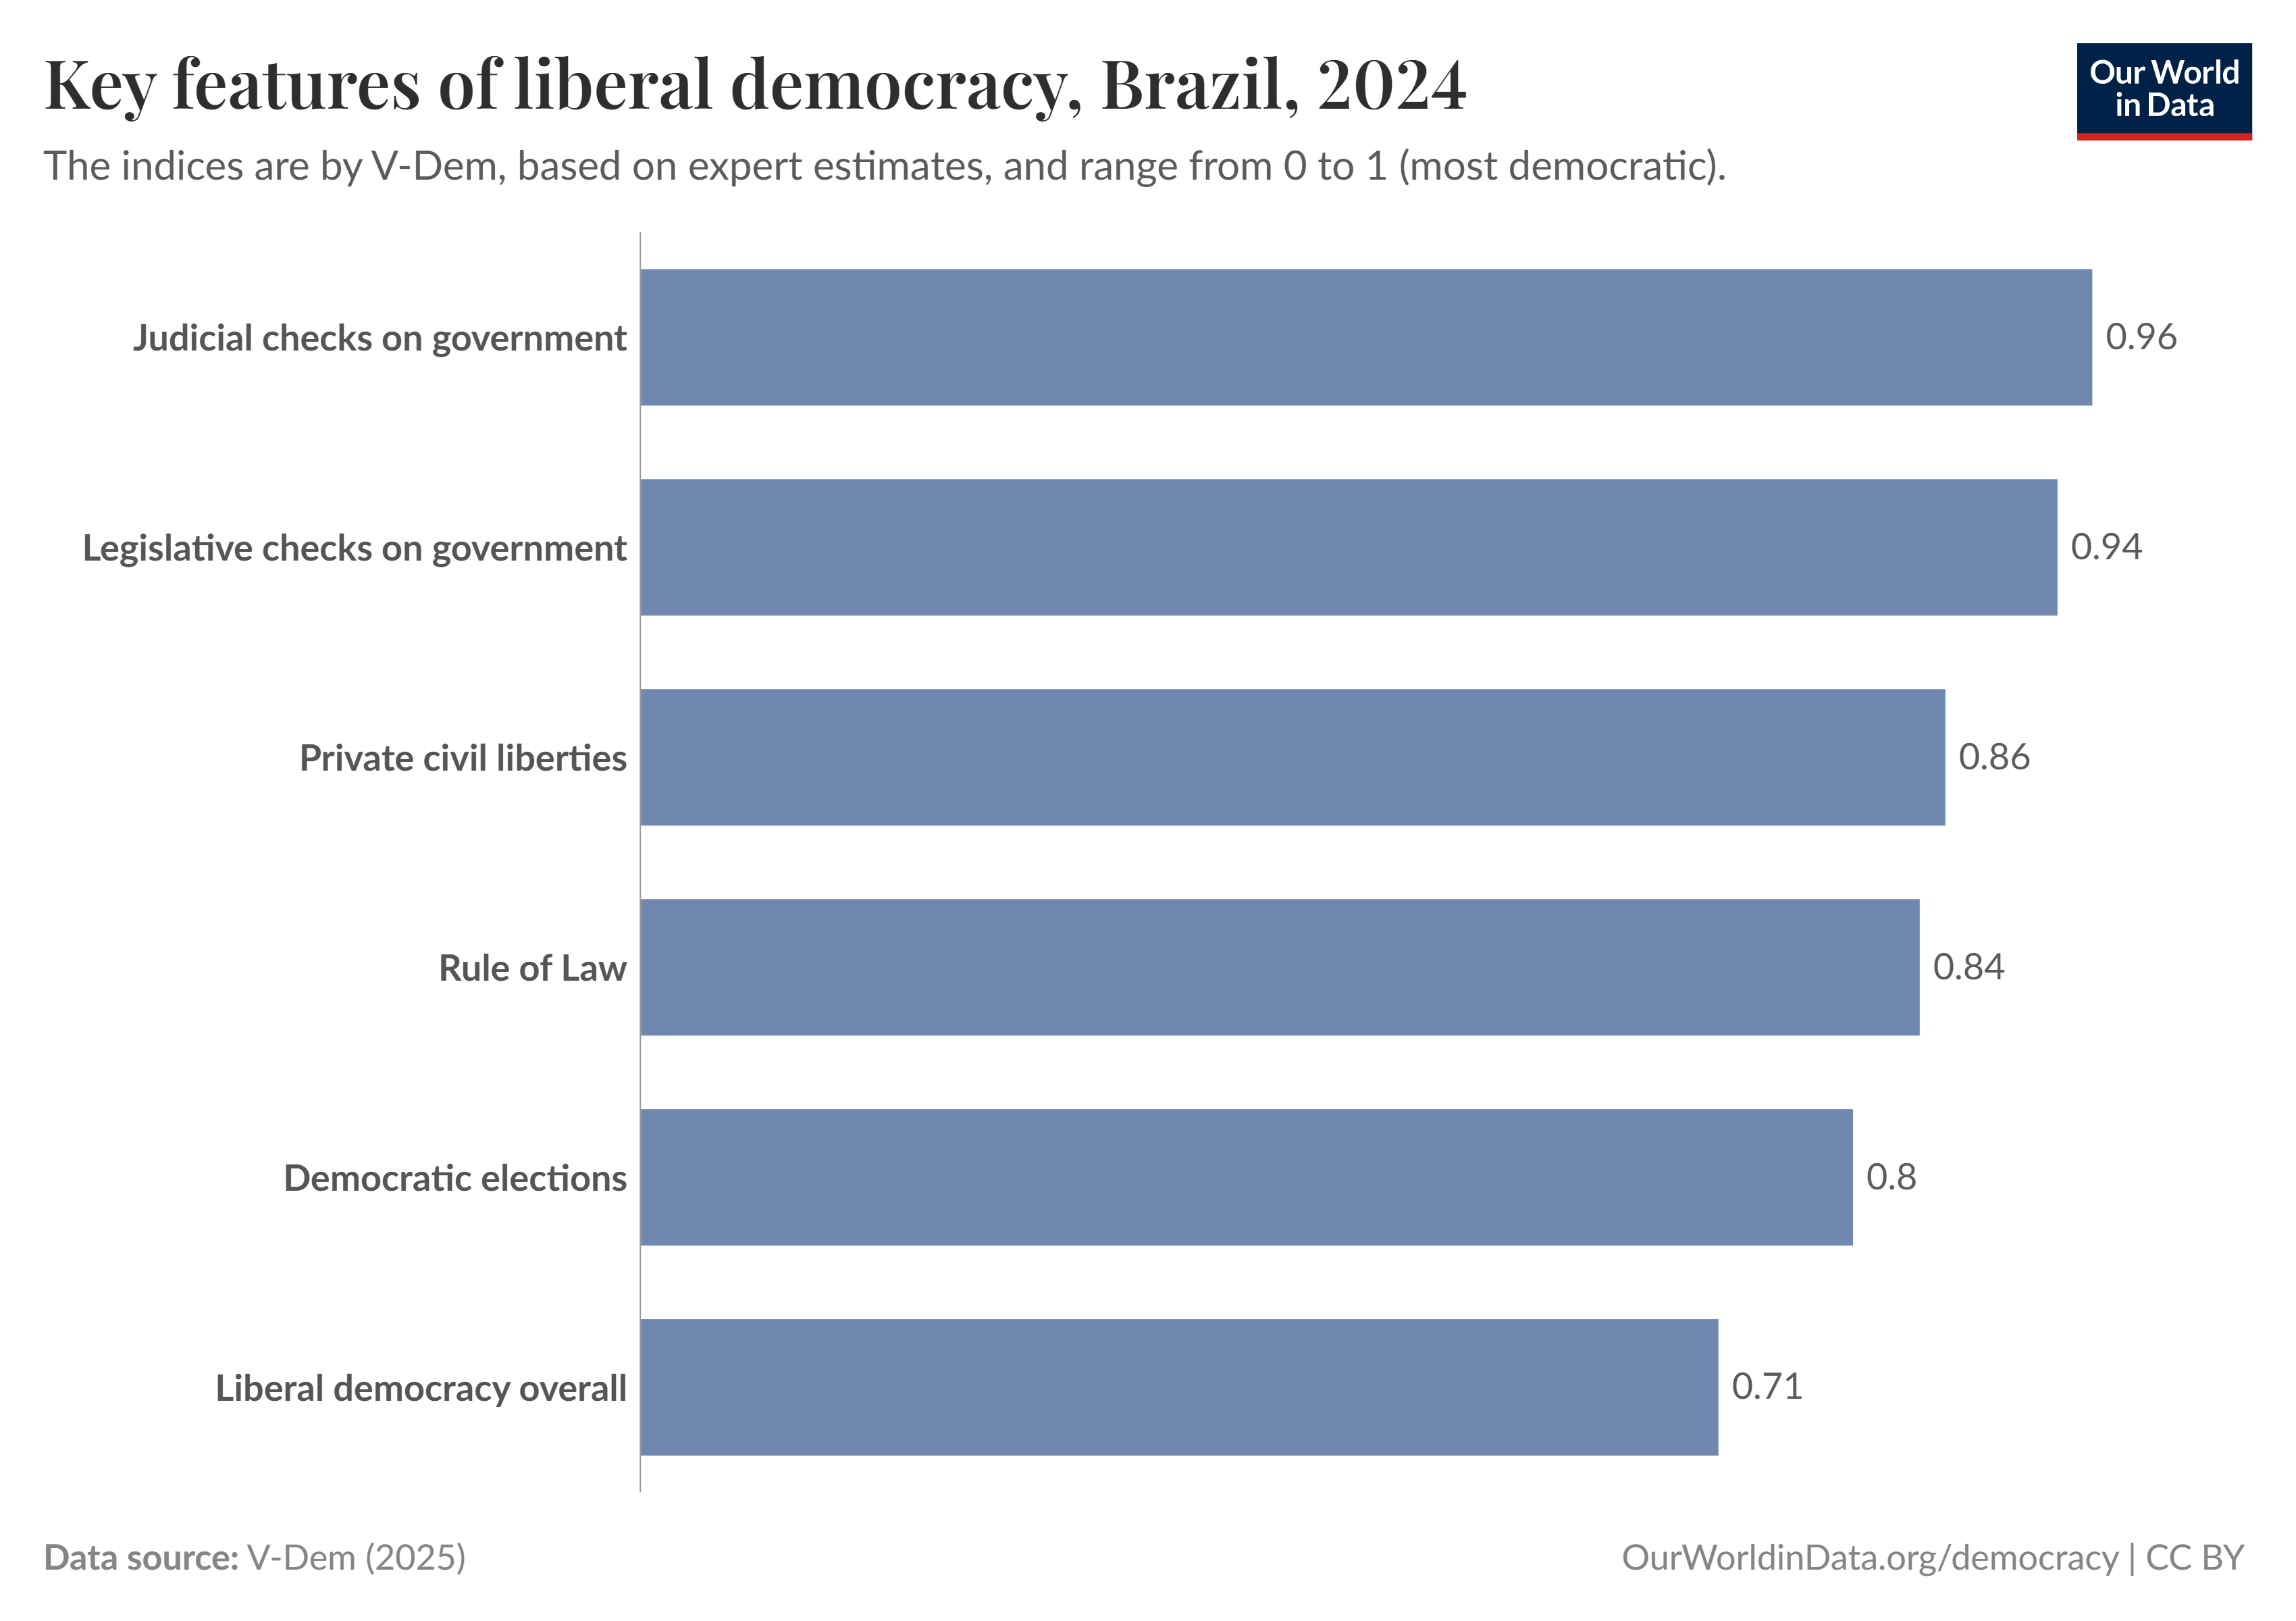
\includegraphics[width=1\linewidth]{figuras/key-features-of-liberal-democracy}
	\label{fig:key-features-of-liberal-democracy}
	\footnotesize{Fonte: \cite{rule-of-law-index}.}
\end{figure}

Como expresso pela figura \ref{fig:key-features-of-liberal-democracy}, além do controle judicial sobre o Poder Executivo e o Estado de Direito já citados em parágrafos anteriores, o controle legislativo sobre o Poder Executivo, as liberdades civis, as eleições democráticas são altas.

No tocante à liberdade de expressão e associação, bem como, as liberdades civis, a figura \ref{fig:comparacao_liberdade_expressao_associacao_dh}.
.
\begin{figure}[H]
	\centering
	\caption{Índice de liberdade de expressão, liberdade de associação e de liberdades civis no Brasil e a média mundial em 2024}
	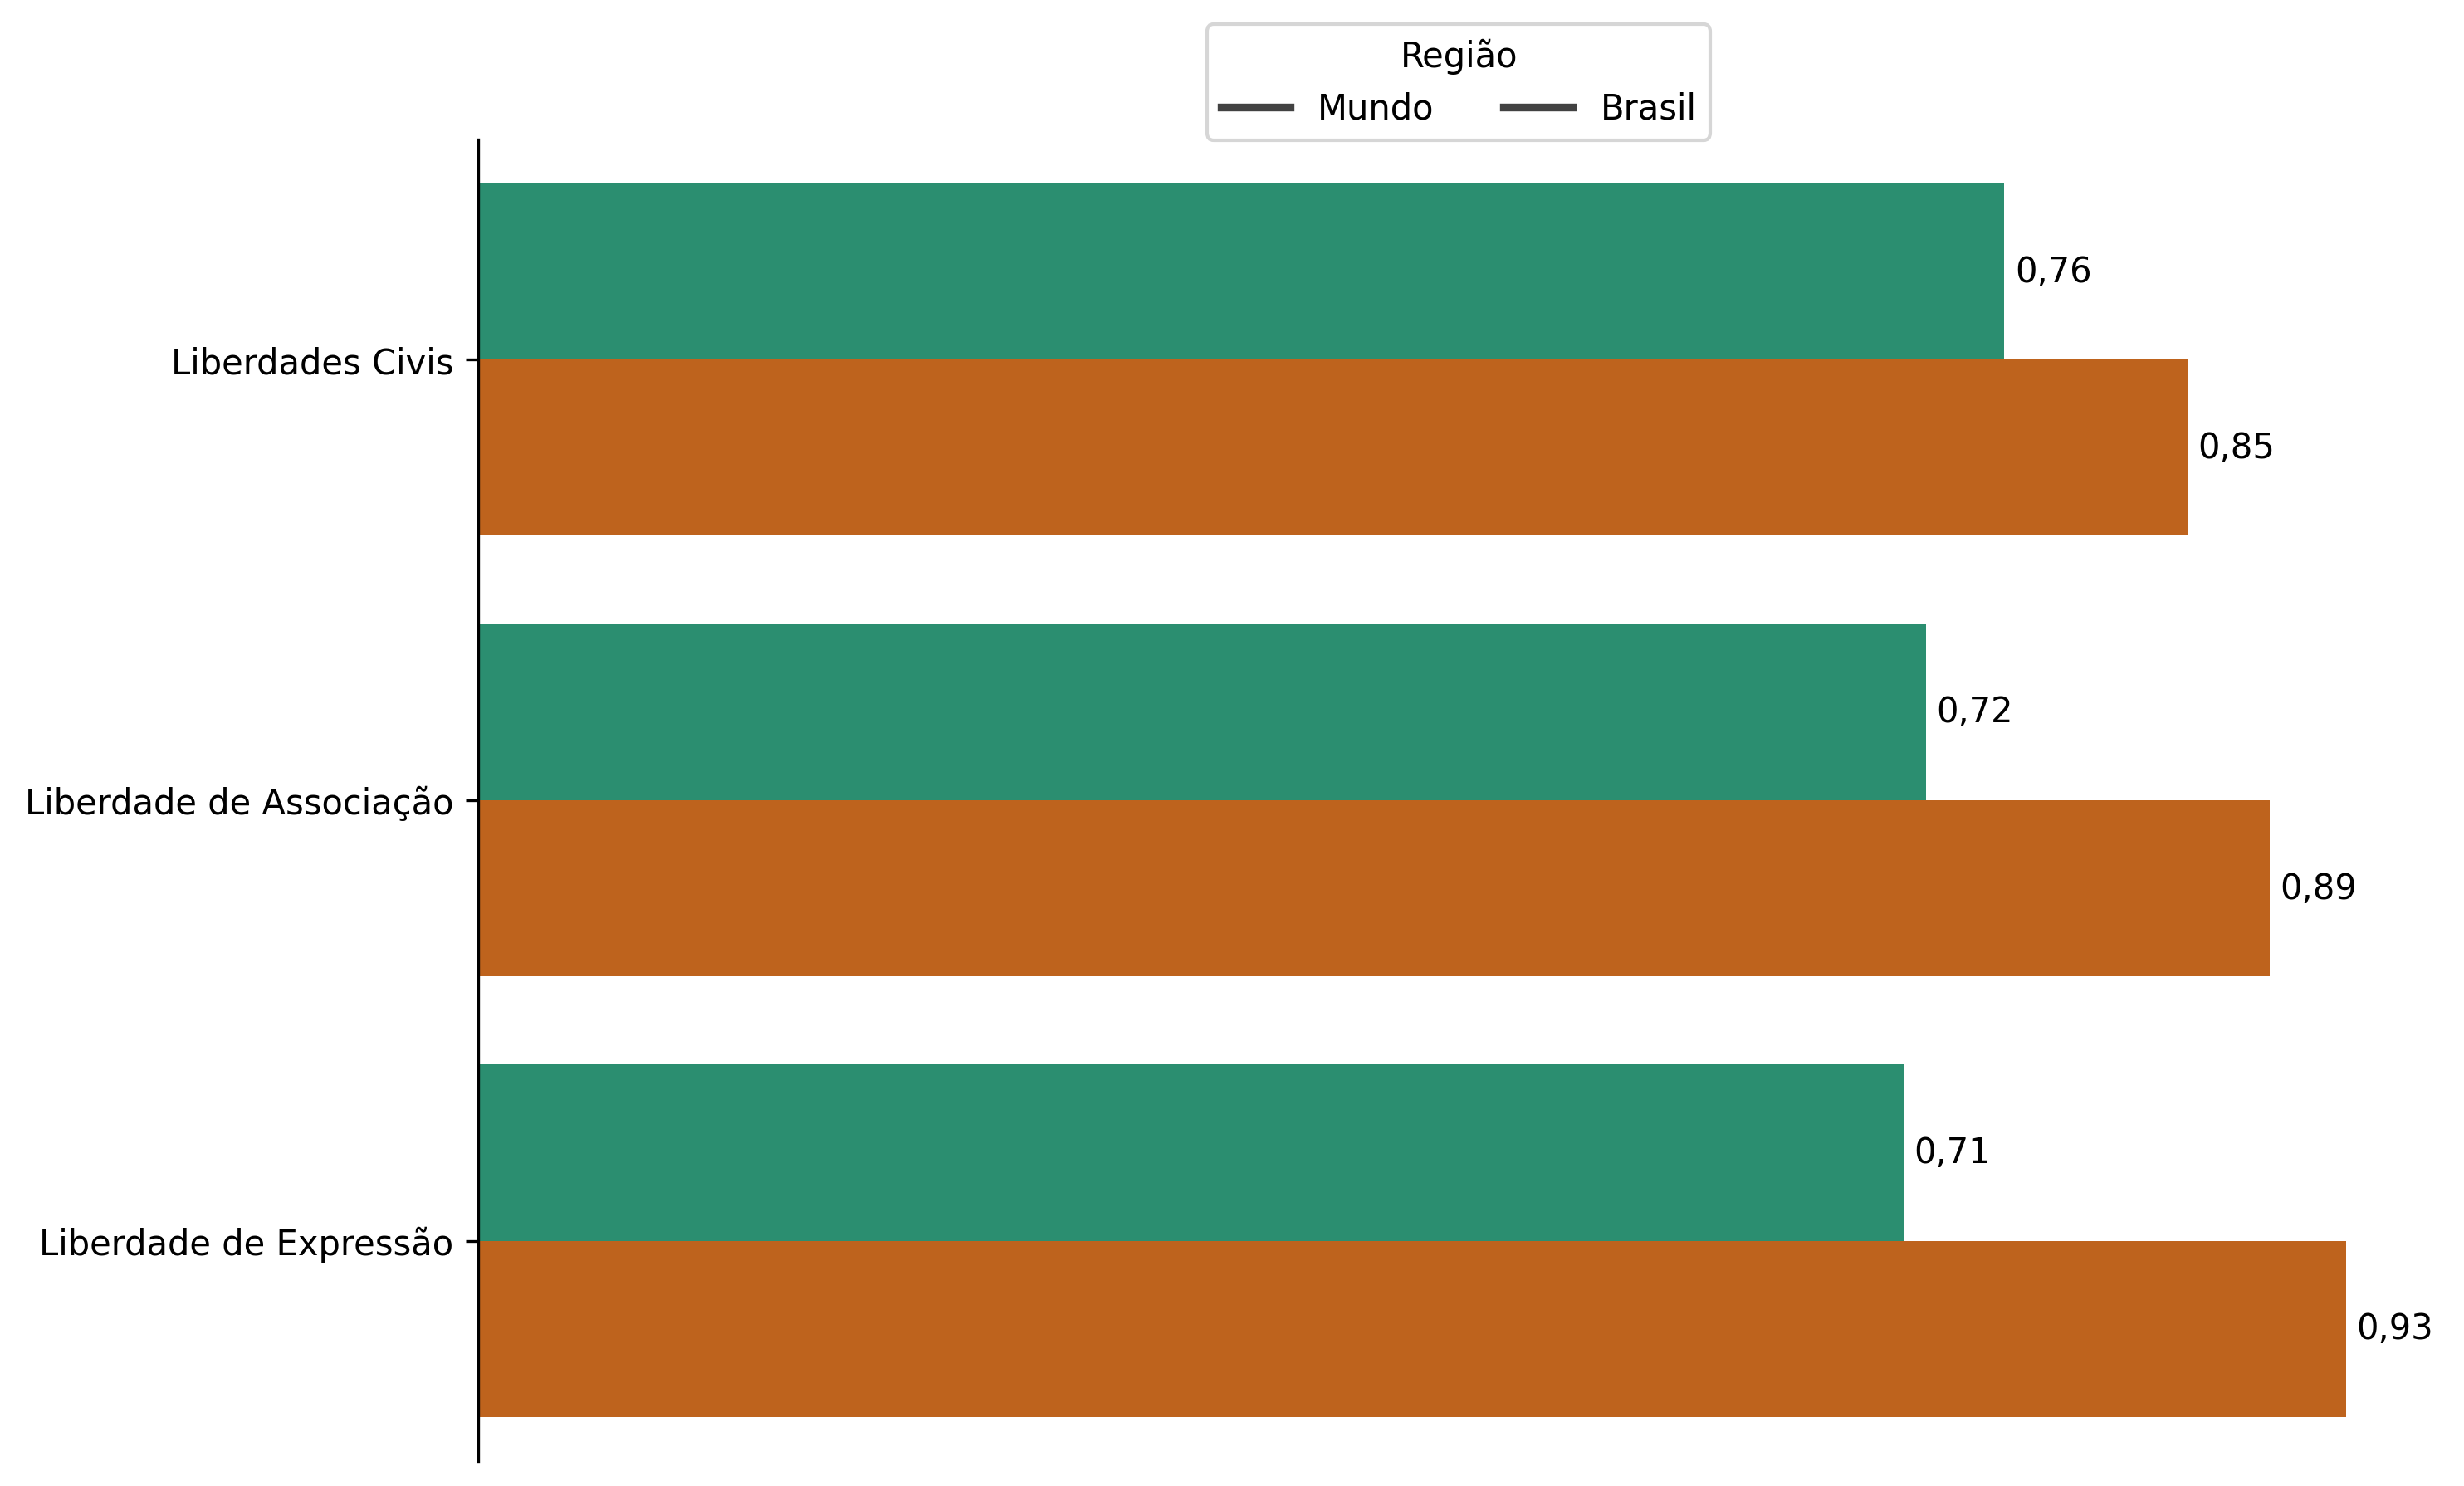
\includegraphics[width=1\linewidth]{figuras/comparacao_liberdade_expressao_associacao_dh}
	\label{fig:comparacao_liberdade_expressao_associacao_dh}
	\footnotesize{Fonte: elaboração própria baseada em \cite{freedom-of-association-index}, \cite{freedom-of-expression-index} e \cite{human-rights-index-vdem}.}
\end{figure}

Conforme expresso na figura \ref{fig:comparacao_liberdade_expressao_associacao_dh}, o Brasil se destaca nos quesitos liberdade de expressão e associação, bem como, os direitos humanos em relação à média mundial.

Os tópicos citados nas figuras \ref{fig:key-features-of-liberal-democracy} e \ref{fig:comparacao_liberdade_expressao_associacao_dh} representam temas ligados à Constituição Federal de 1988. Um exemplo é direito de associação, presente no art. 5º, XVII da Carta Magna, conforme \cite{cf88}, declara como plena a liberdade de associação para fins lícitos, vedada a de caráter paramilitar. O art. 37, VI, nos termos da Constituição, haja vista \cite{cf88}, garante ao servidor público civil o direito à livre associação sindical.

Outro exemplo é o do controle legislativo sobre o Poder Executivo. A Constituição Federal de 1988 concedeu ao Congresso Nacional, com auxilio do Tribunal de Contas da União, haja vista \cite{cf88}, poder fiscalizador sob o Poder Executivo via comissões permanentes, temporárias, especiais e as de inquérito parlamentar.

A Constituição Federal de 1988, assim argumentado por \cite{cf88}, concedeu competência constitucional para o Congresso Nacional sustar os atos normativos do Poder Executivo que exorbitem do poder regulamentar ou dos limites de delegação legislativa.

Ao Congresso Nacional, segundo \cite{cf88}, cabe sustar os efeitos jurídicos, respeitados os direitos adquiridos, de medidas provisórias expedidas pelo Presidente da Republica. E, por fim, conduzir a remoção do cargo de Presidente da República do seu ocupante.

As informações alarmantes apresentadas por \cite{nord2025democracy} expõem o quão benéfica tem sido a democracia para o Brasil desde a redemocratização. Embora o Brasil ainda apresente desafios, o país está em processo de melhoria institucional. Um exemplo disso é o fato do Brasil ter tido a capacidade de reverter uma tentativa de autocratização enquanto 40\%  da população mundial vive em países que estão em processo de autocratização.

Como consequência da argumentação anterior, \cite{pires2021paradoxo} corrobora a independência do Poder Judiciário. Para o autor, o Poder Judiciário obteve níveis elevados de independência com a Constituição Federal de 1988, que em um esforço para fortalecer a independência individual dos juízes, os termos e condições de mandato foram significativamente aprimorados.  Bem como, a Constituição Federal também fortaleceu a independência funcional do judiciário como instituição de governança, isolando-o do sistema político mais amplo.

No tocante aos direitos humanos, algumas decisões de caráter nacional foram aprovadas. Na ADPF 527, de acordo com \cite{adpf527}, "Assim, com base em diálogo institucional estabelecido com o Poder Executivo, como explicitado acima, ajusto os termos da cautelar já deferida para outorgar às transexuais e travestis com identidade de gênero feminina o direito de opção por cumprir pena: (i) em estabecimento prisional feminino; ou (ii) em estabelecimento prisional masculino, porém em área reservada, que garanta a sua segurança."

Outra decisão afeta aos direitos é a jurisprudência do Superior Tribunal de Justiça (STJ) em relação a interpretação judicial e a aplicação do art. 318-A do Código de Processo Penal (CPP), introduzido pela Lei nº 13.769, de 2018, haja vista \cite{cpp}:

\noindent
\begin{flushleft}
\setlength{\leftskip}{4cm}
\small
"Art. 318-A.  A prisão preventiva imposta à mulher gestante ou que for mãe ou responsável por crianças ou pessoas com deficiência será substituída por prisão domiciliar, desde que: (Incluído pela Lei nº 13.769, de 2018).

I - não tenha cometido crime com violência ou grave ameaça a pessoa;              (Incluído pela Lei nº 13.769, de 2018).

II - não tenha cometido o crime contra seu filho ou dependente. (Incluído pela Lei nº 13.769, de 2018)." \cite{cpp}
\end{flushleft}

Visando a plena garantia dos direitos humanos por mulheres que são mães ou responsáveis legais, o STJ tem diversas decisões que usaram o art. 318-A do CPP. 

O RHC 145.931/MG, de 2021, aplicou o art. 318-A do CPP, cujo texto da ementa segue abaixo:

\noindent
\begin{flushleft}
\setlength{\leftskip}{4cm}
\small
"RECURSO EM HABEAS CORPUS. EXECUÇÃO PENAL.	EXECUÇÃO DE PENA PRIVATIVA DE LIBERDADE DE 9 ANOS DE RECLUSÃO. REGIME INICIAL FECHADO. CONDENAÇÃO PELA PRÁTICA DOS CRIMES DE TRÁFICO DE DROGAS E ASSOCIAÇÃO PARA O TRÁFICO. PRETENSÃO DE CONCESSÃO DE PRISÃO DOMICILIAR. PACIENTE GENITORA DE CRIANÇAS DE 6 E 2 ANOS DE IDADE. POSSIBILIDADE. CARACTERIZADA INEFICIÊNCIA ESTATAL EM DISPONIBILIZAR VAGA À RECORRENTE EM ESTABELECIMENTO PRISIONAL PRÓPRIO E ADEQUADO À SUA CONDIÇÃO PESSOAL, DOTADOS DE ASSISTÊNCIA MÉDICA PRÉ-NATAL E PÓS-PARTO, BERÇÁRIOS E CRECHES. ARTS. 82, § 1º, E 83, § 2º, DA LEP. PRESÍDIO FEMININO MAIS PRÓXIMOS DISTANTE 230 KM DA RESIDÊNCIA. CONVIVÊNCIA E AMAMENTAÇÃO IMPOSSIBILITADA. PROTEÇÃO INTEGRAL À CRIANÇA. PRIORIDADE. HC COLETIVO STF N. 143.641/SP. PRECEDENTES DO STJ. LIMINAR DEFERIDA. PARECER MINISTERIAL PELA CONCESSÃO DA ORDEM, EM MENOR EXTENSÃO, A FIM DE QUE A CORTE DE JUSTIÇA SEJA INSTADA A EXAMINAR O MÉRITO DO WRIT IMPETRADO NAQUELA INSTÂNCIA NO TOCANTE À TESE ALEGADA NA INICIAL DA AÇÃO MANDAMENTAL. ILEGALIDADE MANIFESTA 	EVIDENCIADA. RECURSO PROVIDO." \cite{rhc145931}
\end{flushleft}

Evidencia-se da análise da ementa que a mulher julgada foi está sendo condenada por tráfico de drogas e associação ao tráfico, porém na condição de genitora de duas crianças de 2 e 6 anos, foi-lhe concedida a possibilidade de responder em prisão domiciliar, conforme é demostrado abaixo:

\noindent
\begin{flushleft}
\setlength{\leftskip}{4cm}
\small
"2. Ademais, o CPP (com as alterações promovidas pela Lei nº 13.769/2018) passou a prever a substituição da prisão preventiva  por domiciliar à mulher gestante, mãe ou responsável por crianças ou pessoas com deficiência, desde que não tenha cometido crime com violência ou grave ameaça e o delito não tenha sido cometido o crime 	contra seu filho ou dependente, facultando, ainda, a aplicação de medidas cautelares (arts. 318-A e 318-B do CPP)." \cite{rhc145931}
\end{flushleft}

O posicionamento do STJ foi reiterado por outra decisão, a Reclamação nº 40.676/SP.

\noindent
\begin{flushleft}
\setlength{\leftskip}{4cm}
\small
"1. A jurisprudência desta Corte tem se orientado no sentido de que deve ser dada uma interpretação extensiva tanto ao julgado proferido pelo Supremo Tribunal Federal no Habeas Corpus coletivo n. 143.641, que somente tratava de prisão preventiva de mulheres gestantes ou mães de crianças de até 12 anos, quanto ao art. 318-A do CPP, para autorizar também a concessão de prisão domiciliar às rés em execução provisória ou definitiva da pena, ainda que em regime fechado." \cite{reclamacao40676}
\end{flushleft}

Nota-se como a instância superior da Justiça Comum tem foco na dignidade da pessoas humana ao estabelecer como padrão de julgamento a aplicação plena do art. 318-A do CPP, focando na necessidade dos filhos e dependentes legais das mulheres rés na Justiça Criminal, concomitantemente, na condição de responsável e cuidadora de pessoas das rés de pessoas que delas dependem.

De forma complementar, o STF expediu em 2018 o HC nº 143.641/SP. De acordo com \cite{hc143641}, a determinação da Suprema Corte deu-se devido a reclamação das defensorias públicas dos Estados e da União de que as apenadas estavam sofrendo graves de violações dos direitos como gestantes e que seus filhos estariam sendo afetados por extensão, de modo que suas penas em unidades prisionais poderiam ser substituídas por penas alternativas, ou por estarem em prisão preventiva, seriam absorvidas depois. 
	
Outro fatores que motivaram a reclamação perante o Supremo Tribunal Federal (STF), segundo \cite{hc143641}, foram as condições precárias das unidades prisionais que afetam tanto as apenadas, quanto sua prole. Adicionalmente, as apenas estavam tendo outros direitos que estão sendo desrespeitados, não se podendo penalizá-las pela falta de estrutura estatal adequada para fazê-los valer.

Complementarmente, haja vista \cite{hc143641}, foi argumentado que é o direito de punir, e não o direito à vida, à  integridade e à liberdade individual, que deve ser mitigado. Além disso, os reclamantes destacaram também a vulnerabilidade socioeconômica das mulheres presas preventivamente no Brasil. Requereram, por fim, a concessão da ordem para revogação da prisão preventiva decretada contra todas as gestantes puérperas e mães de crianças, ou sua substituição pela prisão domiciliar

Como resultado da independência proporcionada pela Constituição Federal, \cite{pires2021paradoxo} cita que os tribunais receberam controle total sobre seus assuntos administrativos, pessoais e disciplinares, de modo que o Poder Judiciário obteve controle quase total sobre seu orçamento.

No tocante à liberdade de expressão, \cite{daliberdade} cita que, na condição de um dos mais prestigiados direitos das sociedades democráticas, a liberdade de expressão encontra tutela na Constituição Federal, cujo art. 5º, inciso IV, dispõe que “é livre a manifestação do pensamento, sendo vedado o anonimato”.

Para \cite{daliberdade}, o direito à liberdade de expressão, que possui destacada função na concretização do Estado Democrático, em muitas situações se revela em rota de colisão com outros direitos de mesma hierarquia constitucional, principalmente quando está em jogo a delimitação da sua amplitude. 

Nesse sentido, em concordância com \cite{daliberdade}, Para a Corte Suprema, como visto, as linhas que autorizam restrições ao exercício da liberdade de expressão são bastante estreitas. Nesse contexto, o Tribunal não tem admitido proteção à liberdade de expressão em atos de incitação ao ódio, à intolerância e a violência, assim como tem vedado - para além do campo jurídico - manifestações que denotem conteúdo imoral, devendo, ainda, tal liberdade ser pautada pelo resguardo de outros direitos
fundamentais, como a honra, à intimidade e a privacidade.

Um exemplo da ação do STF foi a equiparação do crime de homofobia com o racismo, com base na Lei nº 7.716, de 1989. Conforme \cite{ado26}:

\noindent
\begin{flushleft}
\setlength{\leftskip}{4cm}
\small
"1. Até que sobrevenha lei emanada do Congresso Nacional destinada a
implementar os mandados de criminalização definidos nos incisos XLI e XLII do
art. 5º da Constituição da República, as condutas homofóbicas e transfóbicas, reais ou
supostas, que envolvem aversão odiosa à orientação sexual ou à identidade de gênero de
alguém, por traduzirem expressões de racismo, compreendido este em sua dimensão
social, ajustam-se, por identidade de razão e mediante adequação típica, aos preceitos
primários de incriminação definidos na Lei nº 7.716, de 08/01/1989, constituindo,
também, na hipótese de homicídio doloso, circunstância que o qualifica, por configurar motivo torpe (Código Penal, art. 121, § 2º, I, “in fine”);" \cite{ado26}
\end{flushleft}

Um exemplo de condenação na 1ª instância do Tribunal Regional Federal da 3ª Região com base na Lei nº 7.716, de 1989, foi a de Leonardo de Lima Borges Lins, conhecido como Léo Lins. Na ação penal movida pelo Ministério Público Federal\footnote{cf. \url{https://pje1g.trf3.jus.br/pje/Processo/ConsultaDocumento/listView.seam?x=25053019073589200000353209545}}, haja vista \cite{condenacao_leolins_trf3} abaixo:

\noindent
\begin{flushleft}
	\setlength{\leftskip}{4cm}
	\small
	"Trata-se de denúncia apresentada pelo MINISTÉRIO PÚBLICO FEDERAL em face de LEONARDO DE LIMA BORGES LINS, pela suposta prática dos delitos previstos no artigo 20, parágrafos 2º e 2º-A da Lei nº 7.719/89, por diversas vezes, na forma do art. 71, caput do Código Penal, assim como no artigo 88, parágrafo 2º da Lei nº 13.146/2015, por diversas vezes, na forma do artigo 71 do Código Penal, tudo em concurso material de crimes nos termos do artigo 69 do mesmo Código.
	
	Narra que o denunciado LEONARDO DE LIMA BORGES LINS, vulgo "LÉO LINS", teria publicado e distribuído na plataforma de streaming YouTube e em redes sociais a ele vinculadas, vídeos com conteúdo preconceituoso e discriminatório contra minorias e vulneráveis, dentre eles um vídeo contendo a gravação da apresentação do show de comédia "stand up" por ele realizado, intitulado 'Léo Lins - PERTURBADOR'." \cite{condenacao_leolins_trf3}
\end{flushleft}

Contundo, Léo Lins foi inocentado em um processo movido pelo Município de Nova Hamburgo (RS) contra ele e a produtora BTZ Produções LTDA. Haja vista \cite{liberdade_expressao_artistica_tjrs} que "O Município de Novo Hamburgo propôs Ação Civil Pública com pedido liminar em face de BTZ Produções Ltda. e Leonardo de Lima Borges Lins (Léo Lins), visando impedir a realização do show de stand-up intitulado “Peste Branca” no Teatro Municipal Paschoal Carlos Magno, agendado para o dia 31 de agosto de 2023, das 20h às 22h."

O motivo da ação civil pública do Município de Nova Hamburgo (RS) contra Léo Lins e a produtora BTZ Produções LTDA está descrito abaixo, \textit{ipsis litteris}:

\noindent
\begin{flushleft}
	\setlength{\leftskip}{4cm}
	\small
	"Contudo, em 24 de agosto de 2023, foi publicado nas redes sociais vídeo de divulgação do evento, no qual o réu Léo Lins ridiculariza e difama o Município de Novo Hamburgo, seus habitantes e autoridades locais, incluindo a Prefeita e o Vereador falecido Sergio Hanich. O vídeo viralizou na cidade e gerou ampla revolta popular. A partir da repercussão, apurou-se que o conteúdo do show “Peste Branca” é marcado por piadas de cunho racista, capacitista, gordofóbico e ofensivo a diversas minorias sociais (indígenas, negros, pessoas com deficiência, entre outros). 
	
	[...] 
	
	Sustentou o autor que permitir a realização do evento em espaço público municipal representaria afronta aos princípios constitucionais da dignidade da pessoa humana e da igualdade, bem como violação ao patrimônio público cultural, considerando o simbolismo do Teatro Municipal." \cite{liberdade_expressao_artistica_tjrs}
\end{flushleft}

O Tribunal de Justiça do Rio Grande do Sul (TJRS), proferidor da sentença favorável às partes rés, alegou alguns fundamentos para o indeferimento do pedido:

\begin{itemize}
	\item Da perda superveniente do objeto e da inadequação da tutela jurisdicional requerida.
	\item Da liberdade de expressão e a vedação à censura prévia.
	\item Da inexistência de dano moral coletivo.
	\item Da autonomia do público e o dever de tolerância democrática.
	\item Da legitimidade da empresa ré.
\end{itemize}

Com relação ao fundamento \textbf{Da liberdade de expressão e a vedação à censura prévia}, o TJRS corroborou com a liberdade de expressão, mesmo em situações em que houve conflitos de direitos: liberdade de expressão contra dignidade da pessoa humana, tal como argumentado por \cite{liberdade_expressao_artistica_tjrs}:

\noindent
\begin{flushleft}
	\setlength{\leftskip}{4cm}
	\small
	"O caso que nos ocupa trata-se de uma complexa colisão entre direitos fundamentais consagrados pela Constituição da República, na qual se enfrenta, de um lado, o princípio da dignidade da pessoa humana, da igualdade e da proteção das minorias, e, de outro, o direito à liberdade de expressão artística e ao direito à crítica social, que inclui, também, a manifestação artística sob a forma de humor, ainda que irreverente ou provocativo.
	
	A liberdade de expressão é um direito central em qualquer regime democrático, sendo consagrada no artigo 5º, inciso IX, da Constituição Federal de 1988, e tem um papel crucial no fortalecimento das instituições democráticas. Porém, como todo direito fundamental, não é absoluto e precisa ser ponderado quando se entra em colisão com outros direitos igualmente fundamentais. Em sua função social, a liberdade de expressão permite que opiniões, valores e informações sejam veiculados, garantindo a pluralidade e o debate necessário para a convivência em sociedade. No entanto, como lembra a doutrina, essa liberdade pode ser restringida apenas quando entrar em conflito com outros direitos igualmente fundamentais.
	
	O direito à dignidade da pessoa humana, previsto no artigo 1º, inciso III, da Constituição, impõe que nenhuma expressão, especialmente se veiculada de forma ampla e pública, possa desrespeitar a integridade moral, física ou psíquica do indivíduo ou de grupos sociais vulneráveis. Esse princípio deve ser interpretado como um valor supremo e tem uma função limitadora, que atua como um limite da liberdade de expressão, principalmente quando esta assume caráter discriminatório, racista, homofóbico, sexista, ou qualquer outra manifestação de discurso de ódio." \cite{liberdade_expressao_artistica_tjrs}
\end{flushleft}

Como fundamentação jurídica da defesa da liberdade de expressão, o TJRS citou a ADI nº 4451, conhecida, segundo \cite{liberdade_expressao_artistica_tjrs}, como a "ADI do Humor". A referida ADI, conforme \cite{adi_4451}:

\noindent
\begin{flushleft}
	\setlength{\leftskip}{4cm}
	\small
	"Decisão: O Tribunal, por unanimidade e nos termos do voto do Relator, julgou procedente o pedido formulado na ação direta, para declarar a inconstitucionalidade do art. 45, incisos II e III, da Lei 9.504/1997, bem como, por arrastamento, do § 4º e do § 5º do mesmo artigo, confirmando os termos da medida liminar concedida. Presidiu o julgamento a Ministra Cármen Lúcia. Plenário, 21.6.2018." \cite{adi_4451}
\end{flushleft}  

Da sustanção dos efeitos jurídicos dos dispositivos legais supracitados, \cite{liberdade_expressao_artistica_tjrs} cita que a ADI nº 4.451 garantiu a liberdade de expressão ampla e protegida, inclusive quando se traduz em formas de humor ácido e irreverente, que, muitas vezes, desafiam as convenções sociais e provocam desconforto nas audiências.

\cite{liberdade_expressao_artistica_tjrs} complementou que a decisão da ADI nº 4.451 teve a sensibilidade de entender as peculiaridades do humor, que por sua natureza pode desafiar normas e causar lides. Concomitantemente, o humor não tem a função de agradar, mas sim provocar reflexão, questionar status quo e, por vezes, expor contradições sociais de forma irônica e ácida.

A Constituição Federal, ao assegurar a liberdade de expressão, também reconhece a importância da crítica social para a manutenção da democracia. O humor, como um dos instrumentos de expressão artística, tem sido uma ferramenta histórica de crítica política e social, capaz de expor e questionar normas e comportamentos estabelecidos.

\cite{liberdade_expressao_artistica_tjrs} finaliza com o seguinte argumento:

\noindent
\begin{flushleft}
	\setlength{\leftskip}{4cm}
	\small
	"Entende-se que a liberdade de expressão artística se insere em um campo onde o autor tem a prerrogativa de explorar temas polêmicos, muitas vezes desafiando convenções morais, políticas e até legais. Nesse sentido, o humorista tem o direito de se expressar de maneira irreverente e provocativa, sem que o Estado ou o Judiciário intervenham de forma prévia ou ostensiva, salvo em casos onde haja uma transgressão evidente aos direitos fundamentais de terceiros.
	
	O que distingue o humor da violência simbólica ou do discurso de ódio é justamente a intenção crítica e a ausência de dolo direto de lesar direitos fundamentais de outra pessoa ou grupo. No caso do humorista Leonardo Lins, como citado, mesmo que parte da sociedade possa entender suas piadas como agressivas ou de mau gosto, isso não pode ser razão suficiente para que haja uma restrição prévia à sua liberdade de expressão, sob pena de instaurar um mecanismo de censura indireta." \cite{liberdade_expressao_artistica_tjrs}
\end{flushleft}

Outra marco foi a declaração de não-recepção pela Constituição Federal de 1988 da Lei nº 5.250, de 1967 - conhecida como Lei da Impressa. O STF aprovou a ADPF 130/DF visando garantir a liberdade de impressa no Brasil. Segundo \cite{adpf130}:

\noindent
\begin{flushleft}
\setlength{\leftskip}{4cm}
\small
"Tirante, unicamente, as restrições que a Lei Fundamental de 1988 prevê para o 'estado de sítio' (art. 139), o Poder Público somente pode dispor sobre matérias lateral ou reflexamente de imprensa, respeitada sempre a ideia-força de que quem quer que seja tem o direito de dizer o que quer que seja. Logo, não cabe ao Estado, por qualquer dos seus órgãos, definir previamente o que pode ou o que não pode ser dito por indivíduos e jornalistas. As matérias reflexamente de imprensa, suscetíveis, portanto, de conformação legislativa, são as indicadas pela própria Constituição, tais como: direitos de resposta e de indenização, proporcionais ao agravo; proteção do sigilo da fonte ("quando necessário ao exercício profissional"); responsabilidade penal por calúnia, injúria e difamação; diversões e espetáculos
públicos; estabelecimento dos "meios legais que garantam à pessoa e à família a possibilidade de se defenderem de programas ou programações de rádio e televisão que contrariem o disposto no art. 221, bem como da propaganda de produtos, práticas e serviços que possam ser nocivos à saúde e ao meio ambiente" (inciso II do § 3º
do art. 220 da CF); independência e proteção remuneratória dos profissionais de imprensa como elementos de sua própria qualificação técnica (inciso XIII do art. 5º); participação do capital estrangeiro nas empresas de comunicação social (§ 4º do
art. 222 da CF); composição e funcionamento do Conselho de Comunicação Social (art. 224 da Constituição)." \cite{ado26}
\end{flushleft}

\cite{stf_caderno_liberdadeexpressao} cita outras julgados do STF relativos à liberdade de expressão no periódico \textbf{Cadernos de Jurisprudência do Supremo Tribunal Federal: Concretizando Direitos Humanos}\footnote{\href{https://www.cnj.jus.br/wp-content/uploads/2024/12/cadernos-stf-liberdadeexpressaoenovastecnologias.pdf}{Liberdade de Expressão, Democracia e Novas Tecnologias}}, tais como o HC nº 82.424, o RE nº 511.961, as ADPF nº 187, 4.815, as ADI nº 5.122, 2.566, 4.451, por exemplo.

\section{Barreiras para a modernização do Poder Judiciário}

Para analisar a situação do Poder Judiciário, utilizar-se-á o indicador \textbf{Rule of Law} do WGI. Para \cite{wgi_dados}, \textbf{Rule of Law} captura percepções sobre até que ponto os agentes confiam e cumprem as regras da sociedade e, em particular, a qualidade da execução de contratos, os direitos de propriedade, a polícia e os tribunais, bem como a probabilidade de crime e violência.

A figura \ref{fig:mapa_coropletico_wgi_rl} contém um mapa coroplético que mostra  o indicador \textbf{Rule of Law} pelo mundo.
 
\begin{figure}[H]
	\centering
	\caption{Rule of Law of WGI no mundo em 2023}
	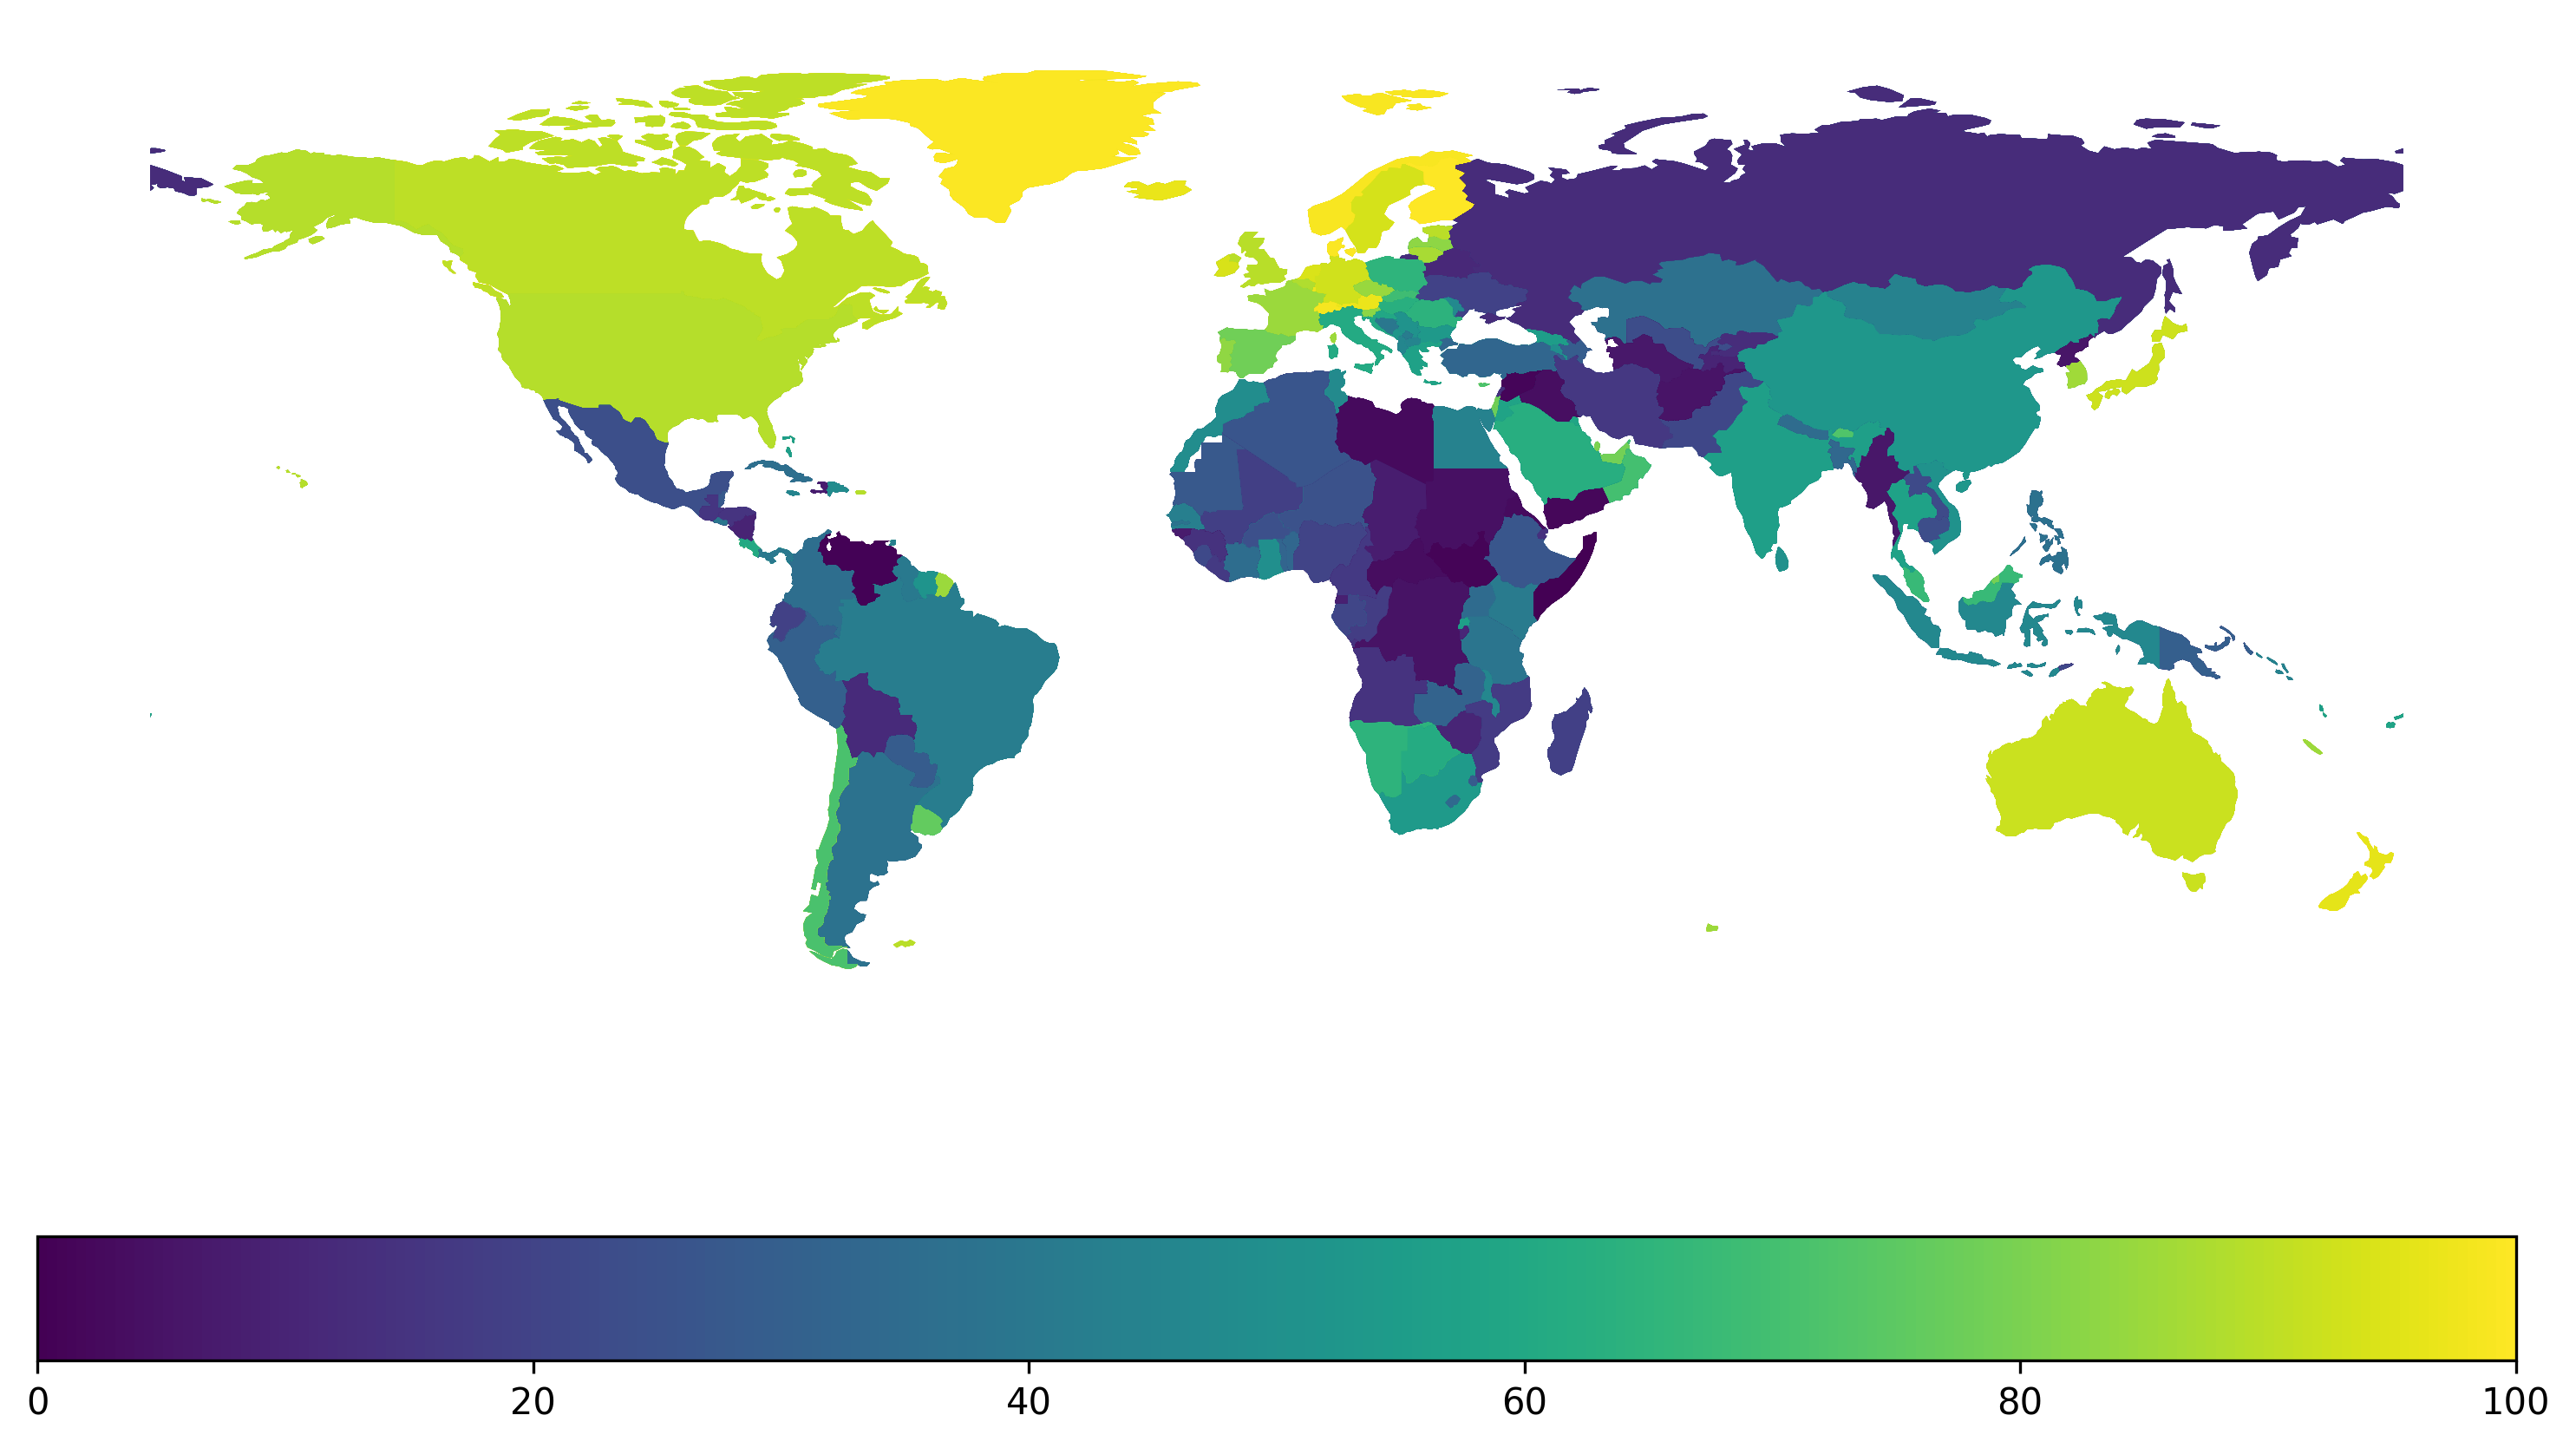
\includegraphics[width=1\linewidth]{figuras/mapa_coropletico_wgi_rl}
	\label{fig:mapa_coropletico_wgi_rl}
	\footnotesize{Fonte: elaboração própria baseada em \cite{wgi_dados}.}
\end{figure}

Nota-se como o Brasil está muito mal posicionado. Até regimes autocráticos como a China, Índia e Arábia Saudita obtiveram um índice melhor. Para entender o histórico global e do Brasil, será demonstrado um gráfico de linha na figura \ref{fig:comparacao_wgi_rl_brasil_mundo}.

\begin{figure}[H]
	\centering
	\caption{Comparação do indicador Rule of Law do WGI do Brasil e do mundo (1996-2023)}
	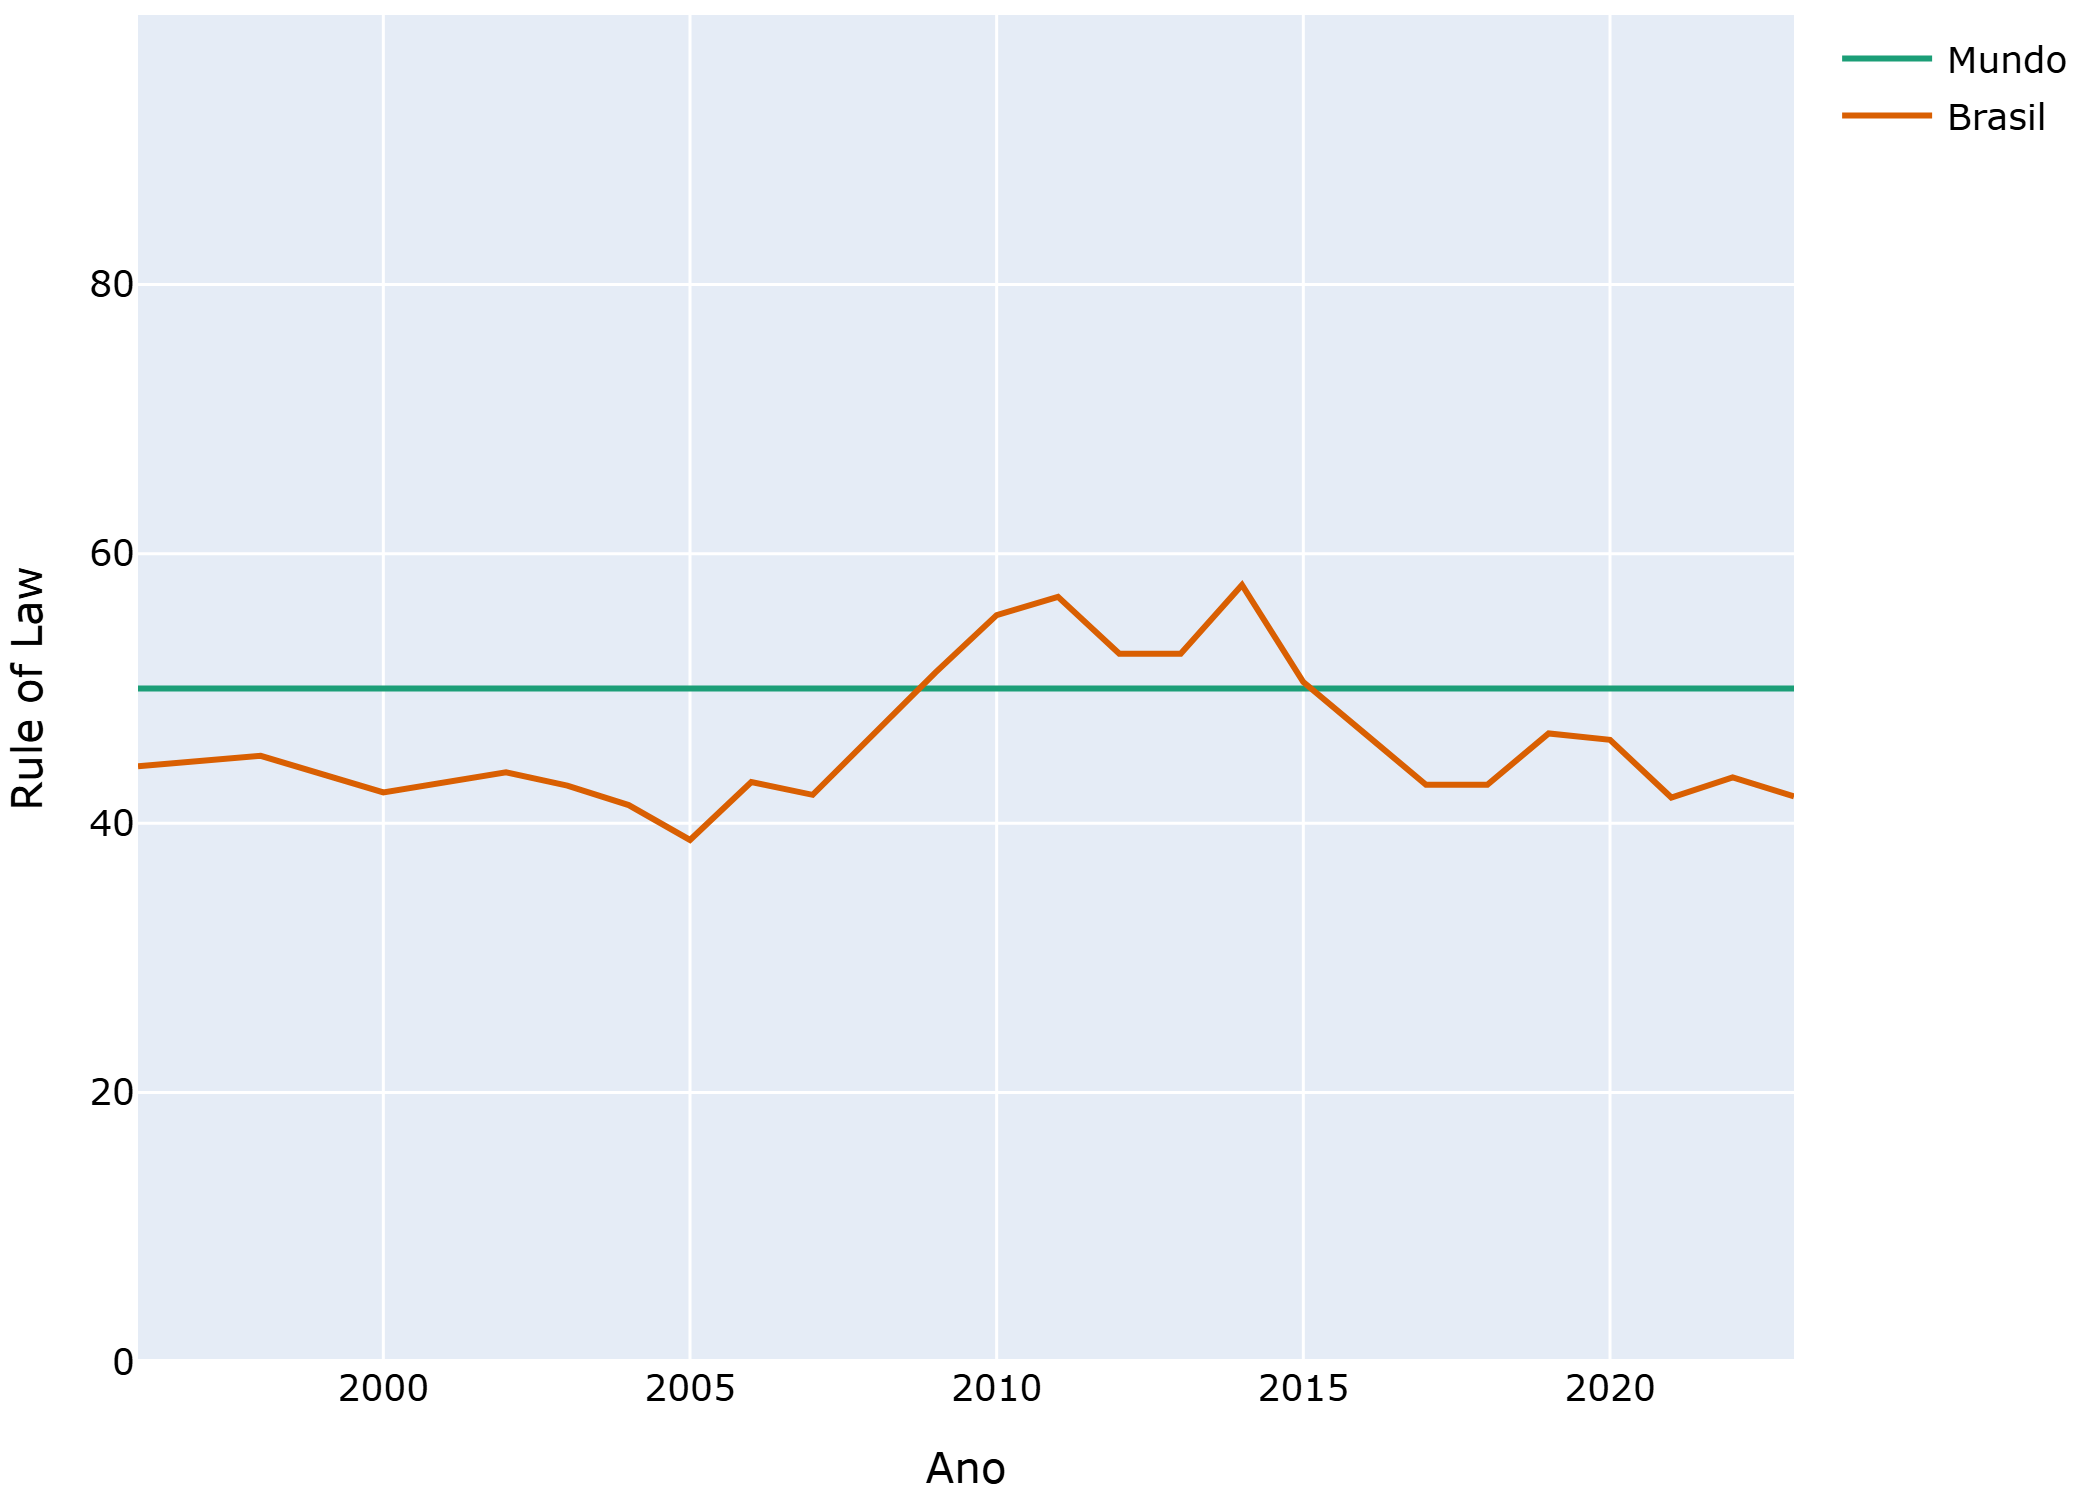
\includegraphics[width=1\linewidth]{figuras/comparacao_wgi_rl_brasil_mundo}
	\label{fig:comparacao_wgi_rl_brasil_mundo}
	\footnotesize{Fonte: elaboração própria baseada em \cite{wgi_dados}.}
\end{figure}

O Brasil teve um breve momento em que ficou à frente da média mundial, porém voltou ao seu padrão baixo de estar em baixo da média. Tal resultado não é exclusivo do Brasil, como exposto pela figura \ref{fig:quartis_wgi_rl}, que contém um gráfico de caixa do indicador \textbf{Rule of Law}.

\begin{figure}[H]
	\centering
	\caption{Gráfico de caixa do Rule of Law do WGI em 2023}
	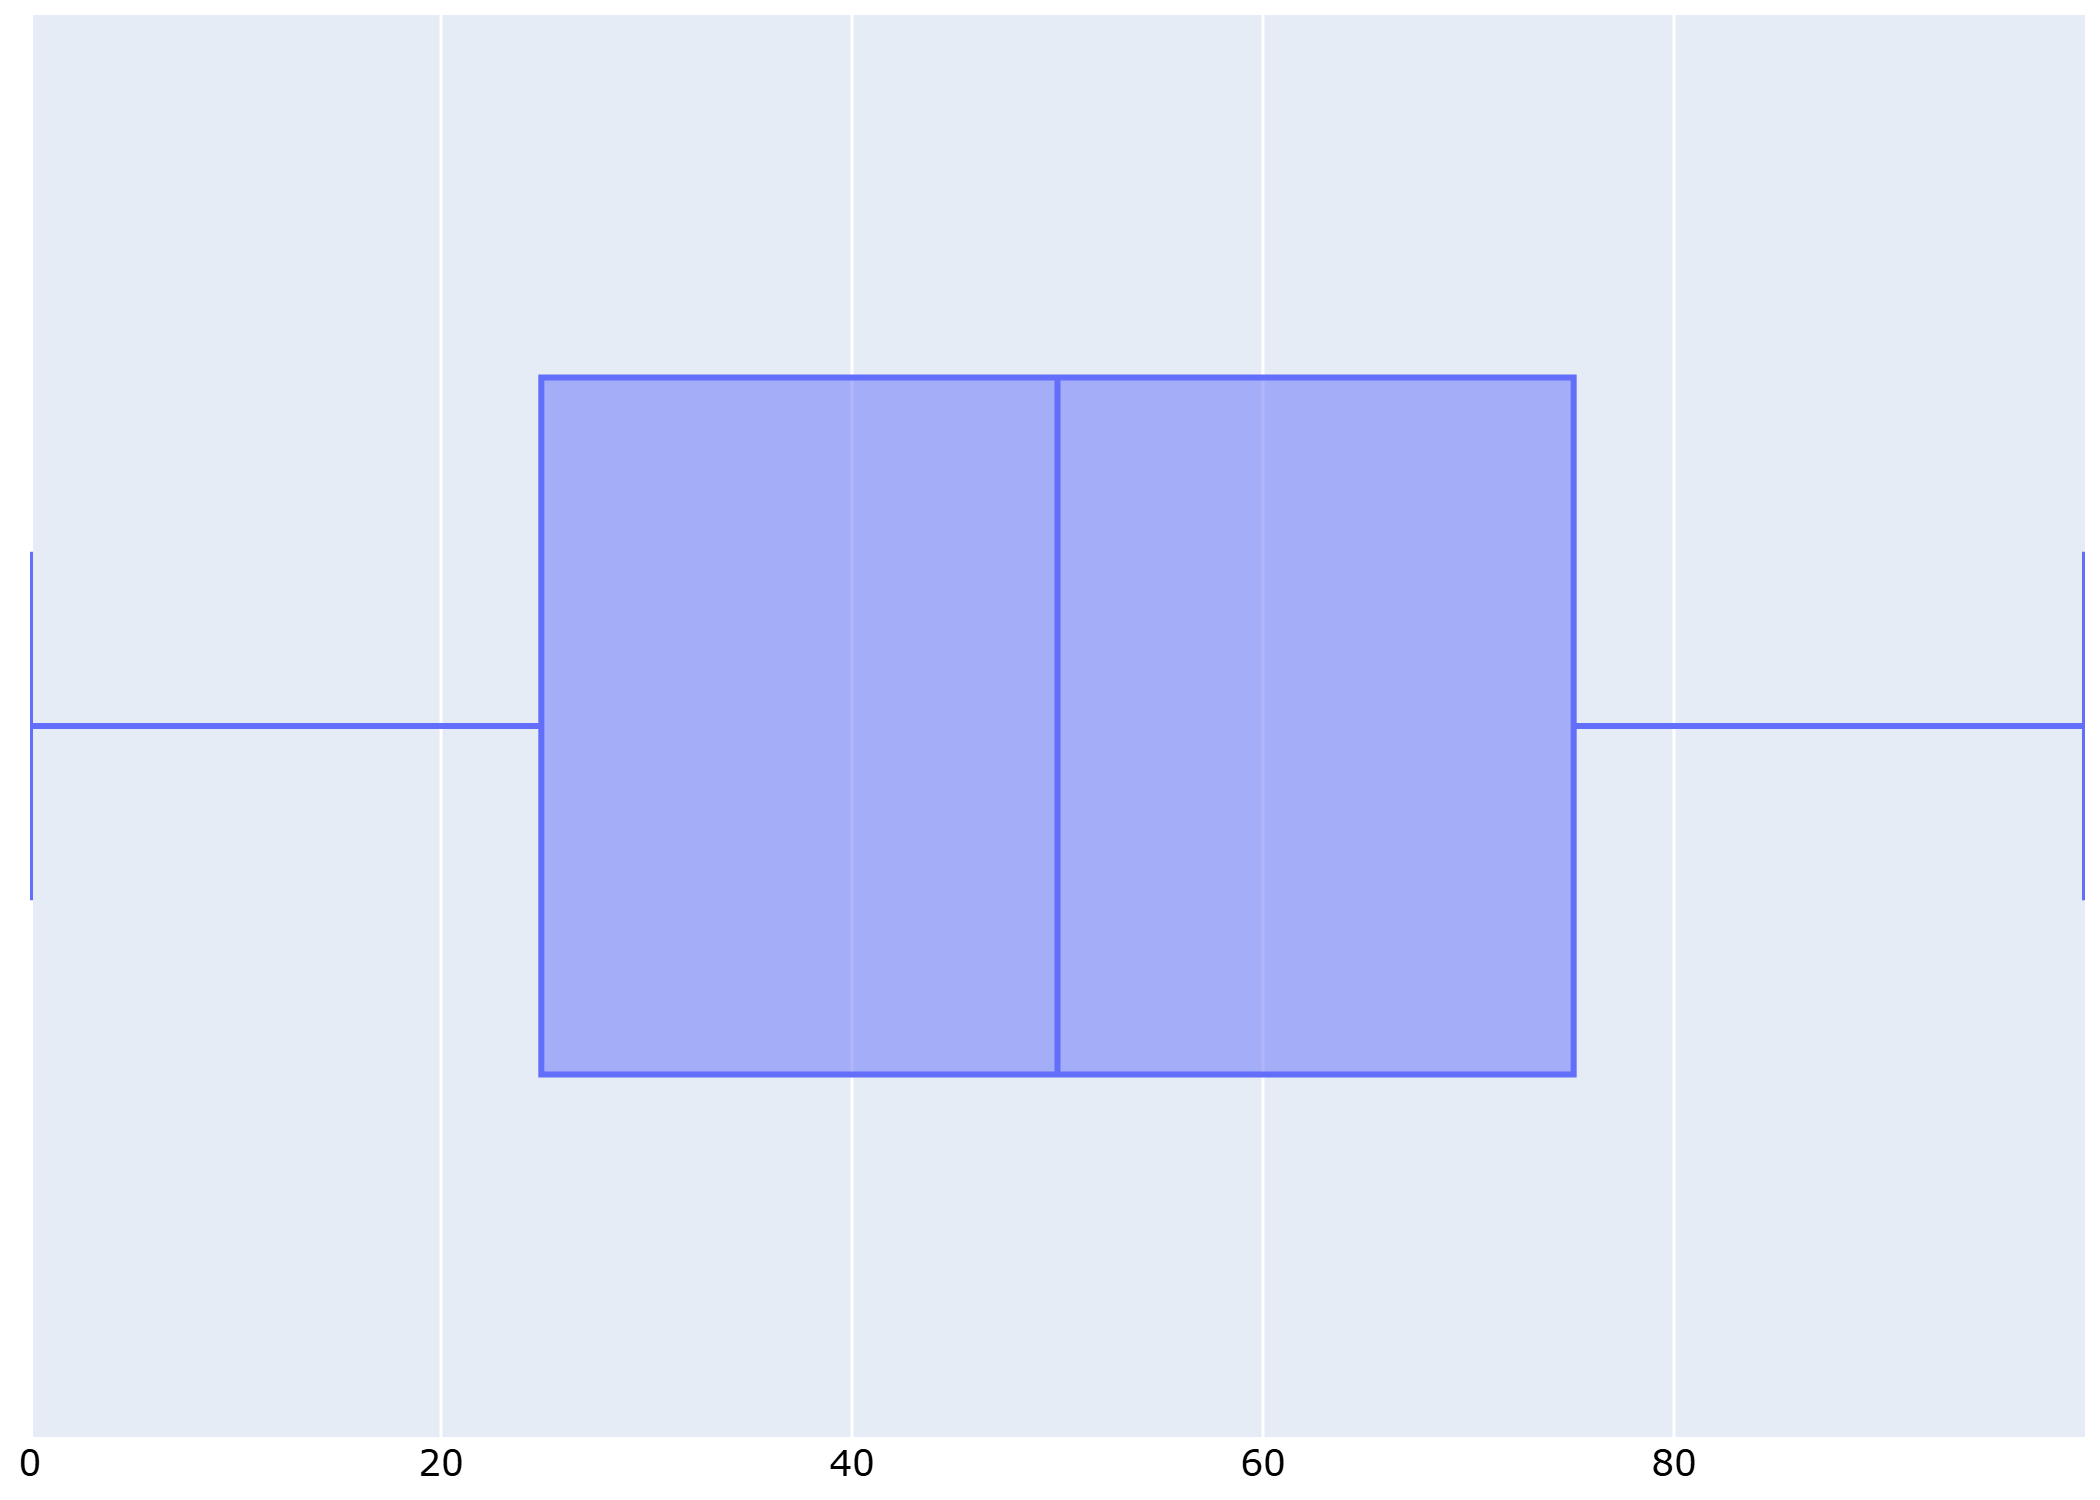
\includegraphics[width=1\linewidth]{figuras/quartis_wgi_rl}
	\label{fig:quartis_wgi_rl}
	\footnotesize{Fonte: elaboração própria baseada em \cite{wgi_dados}.}
\end{figure}

Nota-se pelo equilíbrio da linha central como metade dos países do mundo atingiu menos do que 50\% no indicador \textbf{Rule of Law}. Embora esse problema não seja exclusivo do Brasil e a correlação entre índice de democracia eleitoral e o indicador \textbf{Rule of Law} positivo média (0,6894), os resultados apresentados pelo Brasil na figura \ref{fig:comparacao_wgi_rl_brasil_mundo} demonstram problemas estruturais que barram o avanço da confiança e cumprimento das regras da sociedade pelos agentes e, em particular, a qualidade da execução de contratos, os direitos de propriedade, a polícia e os tribunais, bem como a probabilidade de crime e violência.

\section{Importância da independência do Poder Judiciário}

Como forma de evitar a ingerência do Poder Executivo, \cite{pires2021paradoxo} argumenta que a Constituição Federal estabeleceu o STF é o órgão responsável pela elaboração do orçamento anual da Justiça Federal e pelo encaminhamento direto ao Congresso Nacional. Assim, limitou-se o poder do Governo Federal sob o Poder Judiciário. 

Outro autor destacou a importância da independência do Poder Judiciário foi \cite{akutsu2012dimensoes}. Para ele, a importância de um Poder Judiciário independente dos Poderes Executivo e Legislativo decorre da necessidade de salvaguarda da liberdade individual dos cidadãos, que podem recorrer ao Judiciário contra abusos de autoridades de quaisquer dos três poderes. 

Para \cite{akutsu2012dimensoes}, a independência do Poder Judiciário não deve constituir óbice do cumprimento dos princípios e às normas da Constituição Federal pelos juízes. Além de poder serem responsabilizados perante os cidadãos. 

Complementarmente, para \cite{akutsu2012dimensoes} no caso da premissa da independência dos juízes e tribunais não se concretize, o desempenho do Poder Judiciário pode ser afetado, uma vez que os juízes enfrentariam óbices para  proferir sentenças que desagradassem pessoas afetadas por suas decisões.

Como fortalecedor da independência do Poder Judiciário, e como demonstração constitucional de sua importância para o Brasil, em 2004 o Congresso Nacional aprovou a Emenda à Constituição nº 45, de 2004. \cite{ec45_2004} criou o Conselho Nacional de Justiça (CNJ), as Súmulas Vinculantes do STF, extinguiu os Tribunais de Alçada e determinou sua incorporação aos Tribunais de Justiça, além das outras medidas estabelecidas.

No contexto da mudança legislativa promovida pela  Emenda à Constituição nº 45, de 2004, a criação do CNJ, através da publicação da referida Emenda à Constituição, foi precedida e sucedida de diversas celeumas relaciona das à sua natureza, constitucionalidade, legitimidade e efetividade.

Para \cite{silva2013transparencia}, a criação do CNJ, promovida pela publicação da Emenda à Constituição nº 45, de 2004, foi precedida e sucedida de diversas celeumas relaciona das à sua natureza, constitucionalidade, legitimidade e efetividade.  

Ao CNJ, segundo \cite{silva2013transparencia}, foram concedidos importantes poderes para que o órgão, respondendo do constituinte derivado, respondendo pelo controle da atuação administrativa e financeira do Poder Judiciário.

\section{Modernização do Poder Executivo}   

%Modernização do poder judiciário

Serão discutidos sistemas informatizados criados pelos órgão do Poder Judiciário da União. Os escolhidos foram os seguintes sistemas:

\begin{itemize}
	\item Sistema Eletrônico de Informações (SEI).
	\item Creta
	\item Processo Judicial Eletrônico (PJe)
	\item e-Sistema de Processo Eletrônico (Eproc)
	\item Plataforma Digital do Poder Judiciário Brasileiro (PDPJ-Br)
\end{itemize}

Cada sistema tentou resolver situações pontuais do Poder Judiciário. O SEI tentou modernizar os processos e documentos arquivísticos eletrônicos. O Creta, Eproc e o PJe tentaram modernizar os processos judiciais nos tribunais. O PDPJ-Br tentou modernizar o Poder Judiciária via sua plataforma de acesso único, evitando múltiplos sistemas usados por diferentes tribunais. 

\subsection{Sistema Eletrônico de Informações}

\subsection{Creta}

\subsection{Processo Judicial Eletrônico}

\subsection{e-Sistema de Processo Eletrônico}

\subsection{Plataforma Digital do Poder Judiciário Brasileiro}